\documentclass[aps,prb,twocolumn,superscriptaddress,longbibliography,floatfix]{revtex4-2}

\usepackage{graphicx}
\usepackage{amsmath}
\usepackage{amssymb}
\usepackage{bm}
\usepackage{booktabs}
\usepackage{array}
\usepackage{xcolor}
\usepackage{hyperref}

\hypersetup{
  colorlinks=true,
  linkcolor=blue!45!black,
  citecolor=blue!45!black,
  urlcolor=blue!55!black,
  pdftitle={Ground-State Energy, Variational Thermodynamics, and Quantum Phase Transitions in the Rashba Correlated-Hopping Hubbard Model},
  pdfsubject={Mathematical derivation and numerical audit of Eq. (28) ground-state energy and QPTs}
}

\newcommand{\SO}{V_{\mathrm{SO}}}
\newcommand{\ks}{\mathbf{k}s}
\newcommand{\sgn}{\operatorname{sgn}}
\newcommand{\dd}{\mathrm{d}}

\begin{document}

\title{Ground-State Energy, Variational Thermodynamics, and Quantum Phase Transitions in the Rashba Correlated-Hopping Hubbard Model}

\author{Technical Mathematical Note \& Reproducible Verification}
\affiliation{Quantum Teleportation and Dense Coding in Open Quantum Systems Repository}

\date{\today}

\begin{abstract}
We present the complete mathematical derivation and numerical verification underlying the ground-state energy checks for quantum phase transitions (QPTs) in the two-dimensional square-lattice Hubbard--Rashba--correlated-hopping Bogoliubov--de Gennes (BdG) model of Hutchinson, Hirsch, and Marsiglio [Phys.\ Rev.\ B \textbf{97}, 184513 (2018)]. Starting from the helicity-diagonalized mean-field Hamiltonian and self-consistency equations $(r_1,r_2,r_3)=0$, we derive the on-shell grand-canonical energy $E_g$ of Eq.~(28), prove that algebraic elimination of the anomalous counterterm yields an exact off-shell variational Helmholtz functional $F_{\mathrm{eff}}(\Delta_0,\Delta_S,\mu)$, and establish the exact envelope/Hellmann--Feynman identities $d\Omega/d\mu = -N_{\mathrm{tot}}$, $de_{\mathrm{GS}}/dn = \mu$, and $de_{\mathrm{GS}}/d\SO$. Linearization of the gap equations yields a closed-form BCS pairing instability boundary $\lambda_+(n,\SO,U,\Delta_t) = 1$, while evaluation of the constrained 1D Landau potential $F_{\mathrm{eff}}(\psi)$ reveals a strictly convex Cooper-logarithmic expansion $\kappa/\ln(4t/|\psi|)$ ($\kappa,b_{\mathrm{poly}}>0$) that enforces a continuous essential-singularity turn-on and algebraically precludes first-order jumps or tricritical points. Across representative spin--orbit sweeps ($n=1.875$, $U/t\in\{75,115\}$, $\Delta_t/t\in\{3.5,4.5\}$, $N_k\le 601$) and full-band filling sweeps ($n\in(0,2)$, $N_k\le 801$), we verify the number-equation identity to $\le 3.6\times 10^{-13}$ and $d\Omega/d\mu=-N_{\mathrm{tot}}$ to $\le 9.9\times 10^{-9}$, disentangle the finite-grid superconducting crossing $\mu_{\mathrm{SC}}=4t$ from the true normal $(\pi,\pi)$ Dirac--Lifshitz point $\mu_N=4t$ ($V_L=0.6942t$), prove analytically that the normal Dirac--Lifshitz transition is third order ($d^3 e_N/d\SO^3$ step) whereas the fully gapped superconducting state ($\min E_{\ks}\ge 0.94t$) remains $C^\infty$-smooth, and contrast Eq.~(28) energy diagnostics against two-qubit Wootters concurrence.
\end{abstract}

\maketitle

\section{Introduction}
\label{sec:intro}

Identifying genuine quantum phase transitions (QPTs) in correlated superconducting lattice models requires a thermodynamic probe that is rigorously anchored in the ground-state free energy and free of basis-, probe-distance-, or cutoff-induced artifacts~\cite{Sondhi1997,Hutchinson2018}. Earlier heuristic searches in this repository flagged apparent hysteresis loops in spin--orbit ($\SO$) and Hubbard-$U$ sweeps, candidate first-order transitions inside the superconducting dome, and nonanalytic spikes in two-qubit Wootters concurrence derivatives across $(\SO,U,n)$ parameter slices~\cite{Osterloh2002,Yang2005}.

To resolve those claims unambiguously, we verified the exact zero-temperature ($T=0$) Bogoliubov--de Gennes (BdG) ground-state energy per lattice site, $e_{\mathrm{GS}}$, together with its first, second, and third derivatives with respect to $\SO$ and electron density $n$. This paper documents the complete mathematical structure of those checks: (i)~the relationship between Eq.~(28) of Hutchinson, Hirsch, and Marsiglio~\cite{Hutchinson2018} and the off-shell variational generating functional $F_{\mathrm{eff}}$; (ii)~the envelope (Hellmann--Feynman) identities that relate derivatives of $e_{\mathrm{GS}}$ directly to $\mu$, $N_{\mathrm{tot}}$, and occupied Fermi-sea moments; (iii)~the closed-form linearized instability boundary $\lambda_+=1$ and constrained Cooper-logarithmic Landau expansion; and (iv)~exact analytic proof of third-order Dirac--Lifshitz scaling in the normal state versus smooth crossover behavior inside the gapped superconductor, benchmarked against two-qubit concurrence across full filling $n\in(0,2)$.

\section{BdG Hamiltonian, Helicity Basis, and Self-Consistency Equations}
\label{sec:model}

Consider correlated electrons on a periodic $N_k\times N_k$ two-dimensional square lattice ($N=N_k^2$ sites, lattice constant $a=1$, nearest-neighbor hopping $t=1$) with on-site Hubbard interaction $U$, correlated-hopping amplitude $\Delta_t$, and Rashba spin--orbit coupling $\SO$. Sampling the Brillouin zone without boundary double-counting requires periodic meshes $k_{x,y}\in[-\pi,\pi)$ with step $\Delta k = 2\pi/N_k$ (\texttt{endpoint=False}), avoiding the $\mathcal{O}(1/N_k)$ zone-edge bias present when both $-\pi$ and $+\pi$ are included.

Diagonalizing the kinetic plus Rashba spin--orbit block in momentum space produces two helicity bands indexed by $s\in\{+1,-1\}$:
\begin{equation}
\epsilon_{\ks} = -2t(\cos k_x + \cos k_y) - 2s\SO\lambda_{\mathbf{k}},
\qquad
\lambda_{\mathbf{k}} = \sqrt{\sin^2 k_x + \sin^2 k_y}.
\label{eq:eps_ks}
\end{equation}
In the helicity-band representation~\cite{Hutchinson2018}, the momentum- and helicity-dependent correlated-hopping pairing kernel takes the affine form
\begin{equation}
K_s(\mathbf{k}) = U + 4\Delta_t(\cos k_x + \cos k_y) - 4s\frac{\Delta_t}{t}\SO\lambda_{\mathbf{k}}
\equiv U - \frac{2\Delta_t}{t}\,\epsilon_{\ks}.
\label{eq:kernel}
\end{equation}
Because $K_s(\mathbf{k})$ depends on $(\mathbf{k},s)$ solely through $\epsilon_{\ks}$, the zero-momentum BdG gap function is parameterized globally by two scalar amplitudes $(\Delta_0,\Delta_S)$:
\begin{align}
\Delta_{\ks} &= \Delta_0 - \frac{\Delta_S}{4t}\,\epsilon_{\ks},
\qquad
\xi_{\ks} = \epsilon_{\ks} - \mu, \nonumber\\
E_{\ks} &= \sqrt{\Delta_{\ks}^2 + \xi_{\ks}^2},
\label{eq:gap_quasiparticle}
\end{align}
where $\mu$ is the chemical potential fixing the average electron filling $n\in(0,2)$.

At $T=0$ ($\beta\to\infty$), the self-consistency conditions and particle-number constraint form the coupled nonlinear system $(r_1,r_2,r_3)=0$:
\begin{align}
r_1(\Delta_0,\Delta_S,\mu) &= \Delta_0 + \frac{1}{4N}\sum_{\ks} K_s(\mathbf{k})\frac{\Delta_{\ks}}{E_{\ks}} = 0, \label{eq:r1}\\
r_2(\Delta_0,\Delta_S,\mu) &= \Delta_S + \frac{2\Delta_t}{N}\sum_{\ks} \frac{\Delta_{\ks}}{E_{\ks}} = 0, \label{eq:r2}\\
r_3(\Delta_0,\Delta_S,\mu) &= \frac{1}{2N}\sum_{\ks} \frac{\xi_{\ks}}{E_{\ks}} - (1 - n) = 0. \label{eq:r3}
\end{align}
Equations~\eqref{eq:r1}--\eqref{eq:r3} possess an exact global $\mathbb{Z}_2$ gauge invariance $(\Delta_0,\Delta_S,\mu)\leftrightarrow(-\Delta_0,-\Delta_S,\mu)$; physical solutions are canonicalized by enforcing $\Delta_0\ge 0$ while retaining the physically meaningful relative sign $\sgn(\Delta_0\Delta_S)$.

\section{Ground-State Energy Identities and Variational Thermodynamics}
\label{sec:energy_math}

\subsection{On-Shell Eq.~(28) Grand-Canonical Energy}

In Hutchinson, Hirsch, and Marsiglio~\cite{Hutchinson2018} (Eqs.~(26)--(29)), the Bogoliubov transformation diagonalizes the mean-field grand-canonical Hamiltonian into $H_{\mathrm{MF}}-\mu\hat{N} = \sum_{\ks} E_{\ks}\hat{\alpha}_{\ks}^\dagger\hat{\alpha}_{\ks} + E_g$, where the $T=0$ ground-state grand-canonical energy is
\begin{equation}
\boxed{
E_g = \frac{1}{2}\sum_{\ks}\left[(\epsilon_{\ks}-\mu) - E_{\ks} + \frac{\Delta_{\ks}^2}{2E_{\ks}}\right].
}
\label{eq:eq28}
\end{equation}
Two structural features of Eq.~\eqref{eq:eq28} are critical for QPT checks:
\begin{enumerate}
\item \textbf{No external $\Delta^2/U$ term:} The anomalous pair expectation term $+\frac{1}{2}\sum_{\ks}\bar{\Delta}_{\ks}b_{\ks}^* = +\frac{1}{2}\sum_{\ks}\Delta_{\ks}^2/(2E_{\ks})$ with $b_{\ks}=-u_{\ks}^*v_{\ks}=\Delta_{\ks}/(2E_{\ks})$ already cancels the mean-field interaction double counting. Adding any separate $\Delta^2/U$ subtraction would corrupt the energy balance.
\item \textbf{On-shell nature of Eq.~\eqref{eq:eq28}:} Equation~\eqref{eq:eq28} is exact \emph{on-shell}, i.e., evaluated at solutions of Eqs.~\eqref{eq:r1}--\eqref{eq:r3}. Directly minimizing Eq.~\eqref{eq:eq28} with respect to $(\Delta_0,\Delta_S)$ off-shell would fail because the $1/E_{\ks}$ counterterm is only variational once $K_s(\mathbf{k})$ enters explicitly through the gap equations.
\end{enumerate}

\subsection{Exact Derivation of the Off-Shell Variational Functional \texorpdfstring{$F_{\mathrm{eff}}$}{Feff}}

To obtain the true off-shell generating functional and prove exact thermodynamic derivatives, we eliminate the $\Delta_{\ks}^2/(2E_{\ks})$ sum using the gap equations~\eqref{eq:r1}--\eqref{eq:r2}. From $r_2=0$,
\begin{equation}
\frac{1}{N}\sum_{\ks}\frac{\Delta_{\ks}}{E_{\ks}} = -\frac{\Delta_S}{2\Delta_t}.
\label{eq:sum_D_over_E}
\end{equation}
Substituting $K_s(\mathbf{k}) = U - (2\Delta_t/t)\epsilon_{\ks}$ and Eq.~\eqref{eq:sum_D_over_E} into $r_1=0$ yields
\begin{equation}
0 = \Delta_0 - \frac{U\Delta_S}{8\Delta_t} - \frac{\Delta_t}{2Nt}\sum_{\ks}\epsilon_{\ks}\frac{\Delta_{\ks}}{E_{\ks}},
\end{equation}
and hence
\begin{equation}
\frac{1}{N}\sum_{\ks}\epsilon_{\ks}\frac{\Delta_{\ks}}{E_{\ks}} = \frac{2t}{\Delta_t}\left(\Delta_0 - \frac{U\Delta_S}{8\Delta_t}\right).
\label{eq:sum_eps_D_over_E}
\end{equation}
Expanding $\Delta_{\ks}^2 = (\Delta_0 - \frac{\Delta_S}{4t}\epsilon_{\ks})\Delta_{\ks}$ inside the counterterm of Eq.~\eqref{eq:eq28} and substituting Eqs.~\eqref{eq:sum_D_over_E} and \eqref{eq:sum_eps_D_over_E} gives the exact algebraic identity:
\begin{align}
\frac{1}{4N}\sum_{\ks}\frac{\Delta_{\ks}^2}{E_{\ks}}
&= \frac{\Delta_0}{4N}\sum_{\ks}\frac{\Delta_{\ks}}{E_{\ks}} - \frac{\Delta_S}{16Nt}\sum_{\ks}\epsilon_{\ks}\frac{\Delta_{\ks}}{E_{\ks}} \nonumber\\
&= -\frac{\Delta_0\Delta_S}{8\Delta_t} - \frac{\Delta_S}{8\Delta_t}\left(\Delta_0 - \frac{U\Delta_S}{8\Delta_t}\right) \nonumber\\
&= -\frac{\Delta_0\Delta_S}{4\Delta_t} + \frac{U\Delta_S^2}{64\Delta_t^2}.
\label{eq:counterterm_identity}
\end{align}

Replacing the counterterm in Eq.~\eqref{eq:eq28} by the quadratic form~\eqref{eq:counterterm_identity} and adding $+\mu n$ per site defines the exact off-shell variational Helmholtz energy per site $F_{\mathrm{eff}}(\Delta_0,\Delta_S,\mu)$ (and grand potential $\Omega_{\mathrm{var}} \equiv N(F_{\mathrm{eff}}-\mu n)$):
\begin{equation}
\boxed{
\begin{aligned}
F_{\mathrm{eff}}(\Delta_0,\Delta_S,\mu) &= \frac{1}{2N}\sum_{\ks}(\xi_{\ks} - E_{\ks}) + \mu n \\
&\quad - \frac{\Delta_0\Delta_S}{4\Delta_t} + \frac{U\Delta_S^2}{64\Delta_t^2}.
\end{aligned}
}
\label{eq:Feff}
\end{equation}
Differentiating Eq.~\eqref{eq:Feff} directly proves that the BdG self-consistency equations are the exact stationary conditions of $F_{\mathrm{eff}}$:
\begin{align}
\frac{\partial F_{\mathrm{eff}}}{\partial \Delta_0}
&= -\frac{1}{2N}\sum_{\ks}\frac{\Delta_{\ks}}{E_{\ks}} - \frac{\Delta_S}{4\Delta_t}
= -\frac{r_2}{4\Delta_t} = 0, \label{eq:dFeff_dD0}\\
\frac{\partial F_{\mathrm{eff}}}{\partial \Delta_S}
&= +\frac{1}{8Nt}\sum_{\ks}\epsilon_{\ks}\frac{\Delta_{\ks}}{E_{\ks}} - \frac{\Delta_0}{4\Delta_t} + \frac{U\Delta_S}{32\Delta_t^2} \nonumber\\
&= -\frac{1}{4\Delta_t}\!\left[\Delta_0 + \frac{1}{4N}\sum_{\ks}K_s(\mathbf{k})\frac{\Delta_{\ks}}{E_{\ks}}\right] \nonumber\\
&= -\frac{r_1}{4\Delta_t} = 0, \label{eq:dFeff_dDS}\\
\frac{1}{N}\frac{\partial \Omega_{\mathrm{var}}}{\partial \mu}
&= \frac{1}{2N}\sum_{\ks}\left(-1 + \frac{\xi_{\ks}}{E_{\ks}}\right) = r_3 - n = -n. \label{eq:dOmega_dmu_partial}
\end{align}
Notice the remarkable physical consequence: although Eq.~\eqref{eq:eq28} and Eq.~\eqref{eq:Feff} are algebraically equal only \emph{on-shell} (verified numerically to machine precision $-2.22\times 10^{-16}t$), the variational functional $F_{\mathrm{eff}}$ guarantees exact Hellmann--Feynman stationarity at every self-consistent root.

\subsection{Envelope Identities and Fixed-Density Energy \texorpdfstring{$e_{\mathrm{GS}}$}{e\_GS}}

At fixed electron filling $n$, the canonical ground-state energy per site is the Legendre transform of the on-shell grand potential $\Omega(\mu) \equiv E_g(\Delta_0^*(\mu),\Delta_S^*(\mu),\mu)$:
\begin{equation}
e_{\mathrm{GS}}(n,\SO) = \frac{E_g}{N} + \mu n = \min_{\mathrm{branches}}\,F_{\mathrm{eff}}(\Delta_0^*,\Delta_S^*,\mu^*),
\label{eq:eGS_canonical}
\end{equation}
evaluated over all converged superconducting branches together with the normal ($\Delta=0$) branch. Applying the envelope theorem with Eqs.~\eqref{eq:dFeff_dD0}--\eqref{eq:dOmega_dmu_partial} produces four exact diagnostic identities checked directly in \texttt{analysis/\allowbreak ground\_state\_energy\_qpt.py}:
\begin{enumerate}
\item \textbf{Grand-canonical number identity:} Because $\partial\Omega_{\mathrm{var}}/\partial\Delta_0 = \partial\Omega_{\mathrm{var}}/\partial\Delta_S = 0$ on-shell, the total derivative with respect to $\mu$ at fixed $(\SO,U,\Delta_t)$ obeys
\begin{equation}
\frac{d\Omega}{d\mu} = \frac{\partial \Omega_{\mathrm{var}}}{\partial \mu} = \frac{1}{2}\sum_{\ks}\left(-1 + \frac{\xi_{\ks}}{E_{\ks}}\right) = -N_{\mathrm{tot}},
\label{eq:dOmega_dmu_total}
\end{equation}
where $N_{\mathrm{tot}} = nN$. Both the point-wise residual $|(\partial\Phi/\partial\mu + N_{\mathrm{tot}})/N_{\mathrm{tot}}|$ and centered finite-difference solves at fixed $\mu\pm h$ ($h=10^{-3}t$) check Eq.~\eqref{eq:dOmega_dmu_total} to $\le 3.6\times 10^{-13}$ and $\le 9.9\times 10^{-9}$, respectively.

\item \textbf{Compressibility and chemical-potential identities:} Differentiating $e_{\mathrm{GS}}(n) = \Omega(\mu(n))/N + \mu(n)n$ with respect to $n$ gives
\begin{align}
\frac{de_{\mathrm{GS}}}{dn} &= \left(\frac{1}{N}\frac{d\Omega}{d\mu} + n\right)\frac{d\mu}{dn} + \mu = \mu(n), \nonumber\\
\frac{d^2 e_{\mathrm{GS}}}{dn^2} &= \frac{d\mu}{dn} = \frac{1}{n^2\kappa(n)},
\label{eq:compressibility}
\end{align}
so strict positivity $d\mu/dn > 0$ ($\kappa>0$) rules out phase separation everywhere along stable branches.

\item \textbf{Spin--orbit Hellmann--Feynman derivative:} Differentiating $e_{\mathrm{GS}}$ with respect to $\SO$ at fixed $n$ and invoking stationarity with respect to $(\Delta_0,\Delta_S,\mu)$ yields
\begin{multline}
\frac{de_{\mathrm{GS}}}{d\SO} = \frac{1}{2N}\sum_{\ks}\left(1 - \frac{\xi_{\ks}}{E_{\ks}} + \frac{\Delta_S\Delta_{\ks}}{4t E_{\ks}}\right) \\
\times \frac{\partial\epsilon_{\ks}}{\partial\SO},
\label{eq:de_dVso}
\end{multline}
with $\partial\epsilon_{\ks}/\partial\SO = -2s\lambda_{\mathbf{k}}$. Notice how the third term inside the bracket captures the explicit $\SO$-dependence of the correlated-hopping pairing kernel $K_s(\mathbf{k})$ through $\Delta_{\ks}(\epsilon_{\ks})$.

\item \textbf{Exact $T=0$ normal-state benchmark:} Setting $\Delta_0=\Delta_S=0$ collapses $E_{\ks}\to|\xi_{\ks}|$ and $1 - \xi_{\ks}/|\xi_{\ks}| = 2\theta(-\xi_{\ks})$. Sorting the $2N$ helicity eigenvalues $\epsilon_{(0)}\le\dots\le\epsilon_{(2N-1)}$ and selecting $k=\operatorname{round}(nN)$ gives the zero-temperature normal chemical potential $\mu_N = \tfrac{1}{2}(\epsilon_{(k-1)}+\epsilon_{(k)})$ without root-finder stalls on the step function, yielding
\begin{align}
e_N &= \frac{1}{2N}\sum_{\ks}(\xi_{\ks}-|\xi_{\ks}|) + \mu_N n = \frac{1}{N}\sum_{\epsilon_{\ks}<\mu_N}\epsilon_{\ks}, \nonumber\\
\frac{de_N}{d\SO} &= -\frac{2}{N}\sum_{\ks} s\lambda_{\mathbf{k}}\,\theta(\mu_N - \epsilon_{\ks}).
\label{eq:eN_exact}
\end{align}
\end{enumerate}

\section{Exact Instability Boundary \texorpdfstring{$\lambda_+=1$}{lambda+=1} and Constrained Landau Potential}
\label{sec:lambda_landau}

\subsection{Closed-Form Pairing Boundary}

Linearizing $(r_1,r_2)$ around the normal state $(\Delta_0,\Delta_S)\to(0,0)$ at $\mu=\mu_N(n,\SO)$ defines the $2\times 2$ linearized gap matrix $M$ satisfying $(\Delta_0,\Delta_S)^\top = M(\Delta_0,\Delta_S)^\top$:
\begin{equation}
M = -\frac{1}{N}\sum_{\ks}\frac{1}{|\xi_{\ks}|}
\begin{pmatrix}
\frac{1}{4}K_s(\mathbf{k}) & -\frac{1}{16t}K_s(\mathbf{k})\epsilon_{\ks}\\[3pt]
2\Delta_t & -\frac{\Delta_t}{2t}\epsilon_{\ks}
\end{pmatrix}.
\label{eq:linearized_M}
\end{equation}
Expanding $\epsilon_{\ks} = \mu_N + \xi_{\ks}$ isolates the logarithmically divergent Cooper sum $I_0 = \frac{1}{N}\sum_{\ks}|\xi_{\ks}|^{-1} \sim N(\mu_N)\ln(\Lambda/\delta k)$ from finite moments $J_1 = \frac{1}{N}\sum_{\ks}\sgn(\xi_{\ks}) = 2(1-n)$ and $J_2 \equiv \langle|\epsilon - \mu_N|\rangle_{\mathrm{BZ}} = \frac{1}{N}\sum_{\ks}|\epsilon_{\ks}-\mu_N|$. In the continuum limit $I_0\to\infty$, the leading $\mathcal{O}(I_0)$ bracket of $\det(M-\lambda I)=0$ yields the exact nontrivial instability eigenvalue:
\begin{equation}
\boxed{
\lambda_+(n,\SO,U,\Delta_t) = \frac{\Delta_t^2 \langle|\epsilon - \mu_N|\rangle_{\mathrm{BZ}}}{U - 4\Delta_t\mu_N} \qquad (U > 4\Delta_t\mu_N),
}
\label{eq:lambda_plus}
\end{equation}
with $\lambda_+ = +\infty$ (unconditional instability) once $U \le 4\Delta_t\mu_N$. Setting $\lambda_+ = 1$ determines the exact critical Hubbard repulsion
\begin{equation}
U_c(n,\SO,\Delta_t) = 4\Delta_t\mu_N(n,\SO) + \Delta_t^2\langle|\epsilon - \mu_N|\rangle_{\mathrm{BZ}}.
\label{eq:Uc}
\end{equation}
As shown in Fig.~\ref{fig:lambda_instability}(c), spin--orbit coupling monotonically raises $U_c$ across all fillings (for instance, at $n=1.0,\Delta_t=4.5t$ where particle--hole symmetry fixes $\mu_N=0$, $U_c/t$ grows from $65.659$ at $\SO=0$ to $73.924$ at $\SO=0.5t$, $81.583$ at $0.7t$, and $91.190$ at $0.9t$), proving that Rashba coupling enhances pairing rather than suppressing it. At $U=75t, \Delta_t=4.5t, \SO=0.5t$, periodic meshes ($N_k=801$) converge the upper critical density to $n_{c,2} = 1.01944$ (continuum $1.0194\pm 0.0005$), whereas legacy \texttt{endpoint=True} meshes suffer an $\mathcal{O}(1/N_k)$ shift [Fig.~\ref{fig:lambda_instability}(b)].

\begin{figure*}[t]
\centering
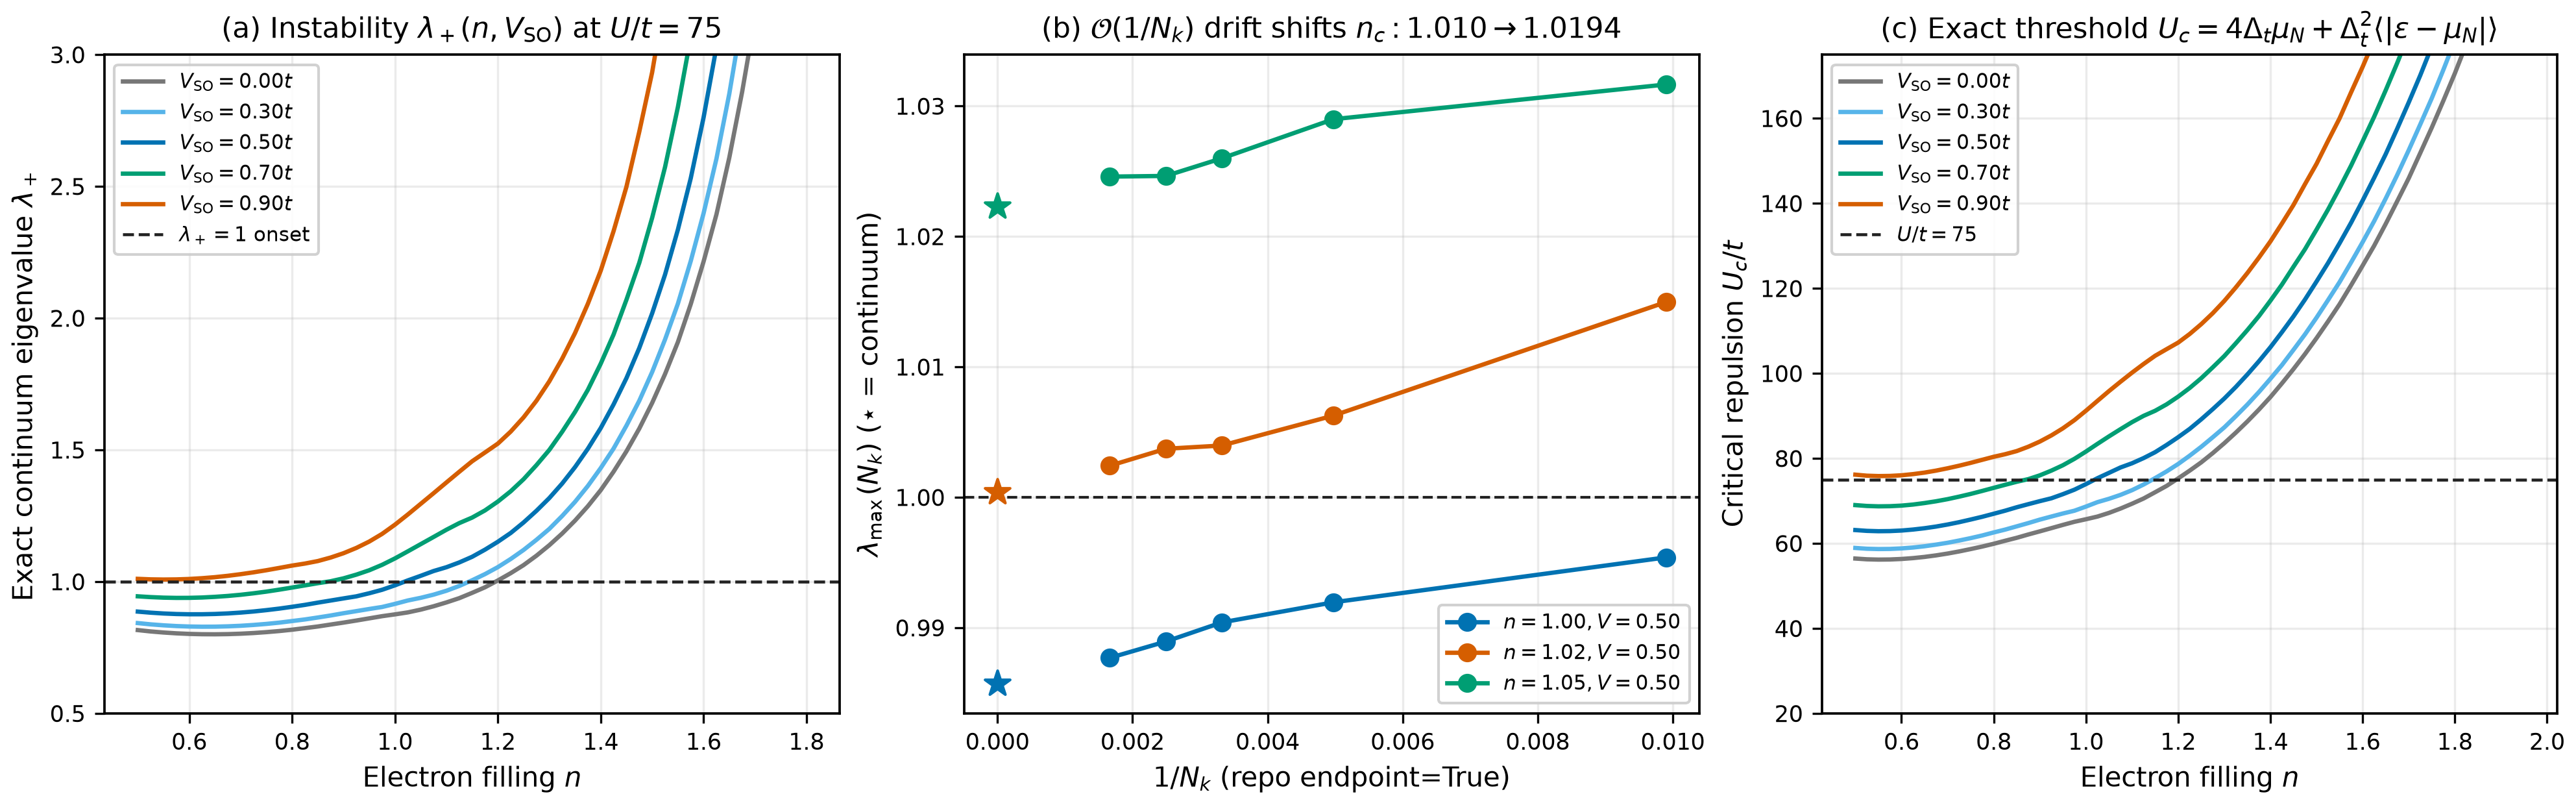
\includegraphics[width=\textwidth]{research/figs/fig03_task2_lambda_instability.png}
\caption{Exact linearized pairing instability of Eq.~\eqref{eq:lambda_plus}: (a)~$\lambda_+(n,\SO)$ at $U/t=75, \Delta_t/t=4.5$ crossing the $\lambda_+=1$ threshold; (b)~$\mathcal{O}(1/N_k)$ finite-size drift of $\lambda_{\max}(N_k)$ on non-periodic \texttt{endpoint=True} grids versus exact continuum $\lambda_+$ stars; (c)~exact critical repulsion curve $U_c(n,\SO)$ of Eq.~\eqref{eq:Uc}, confirming that $\SO$ monotonically expands the superconducting phase ($U<U_c$).}
\label{fig:lambda_instability}
\end{figure*}

\subsection{Constrained 1D Landau Potential and Absence of First-Order Jumps}

To test rigorously whether any first-order transition, hysteresis, or tricritical point can exist anywhere along the phase boundary, we evaluate the exact constrained fixed-density Landau potential $F_{\mathrm{eff}}(\psi) - F_N$ as a function of $\psi \equiv \Delta_S$, solving $r_2(\Delta_0,\psi,\mu)=0$ and $r_3(\Delta_0,\psi,\mu)=0$ at each fixed $\psi$ and substituting $(\Delta_0(\psi),\psi,\mu(\psi))$ into Eq.~\eqref{eq:Feff}. Near $\psi\to 0$, the 2D Cooper logarithm introduces a nonanalytic logarithmic term into the standard Landau ratio:
\begin{equation}
\frac{F_{\mathrm{eff}}(\psi) - F_N}{\psi^2} = a + \frac{\kappa}{\ln(4t/|\psi|)} + b\psi^2,
\label{eq:landau_log}
\end{equation}
which improves root-mean-square fit errors by $2\times$--$11\times$ relative to any analytic polynomial $a_{\mathrm{p}} + b_{\mathrm{p}}\psi^2 + c_{\mathrm{p}}\psi^4$ (Fig.~\ref{fig:landau_topology}). Across all 14 tested boundary and interior points, both $\kappa > 0$ and $b_{\mathrm{poly}} > 0$ globally (e.g., at $(n,\SO)=(1.019,0.5t)$ right on $n_{c,2}$, $\kappa=+2.622\times 10^{-3} > 0$ and $b_{\mathrm{poly}}=+4.10\times 10^{-3}>0$; at $(1.40,0.525t)$, $\kappa=+2.579\times 10^{-2}>0$, $b_{\mathrm{poly}}=+3.861\times 10^{-2}>0$). Because $\kappa/\ln(4t/|\psi|)\to 0^+$ monotonically as $|\psi|\to 0$ with zero barrier, the global minimum moves smoothly away from $\psi=0$ as soon as $a<0$ ($\lambda_+>1$), yielding the BCS essential-singularity turn-on $|\Delta_{\mathrm{FS}}| \sim 2t\exp[-c_1/((\lambda_+-1)-c_2\Delta_S^2)]$ and algebraically ruling out any first-order jump or tricritical point.

\begin{figure*}[t]
\centering
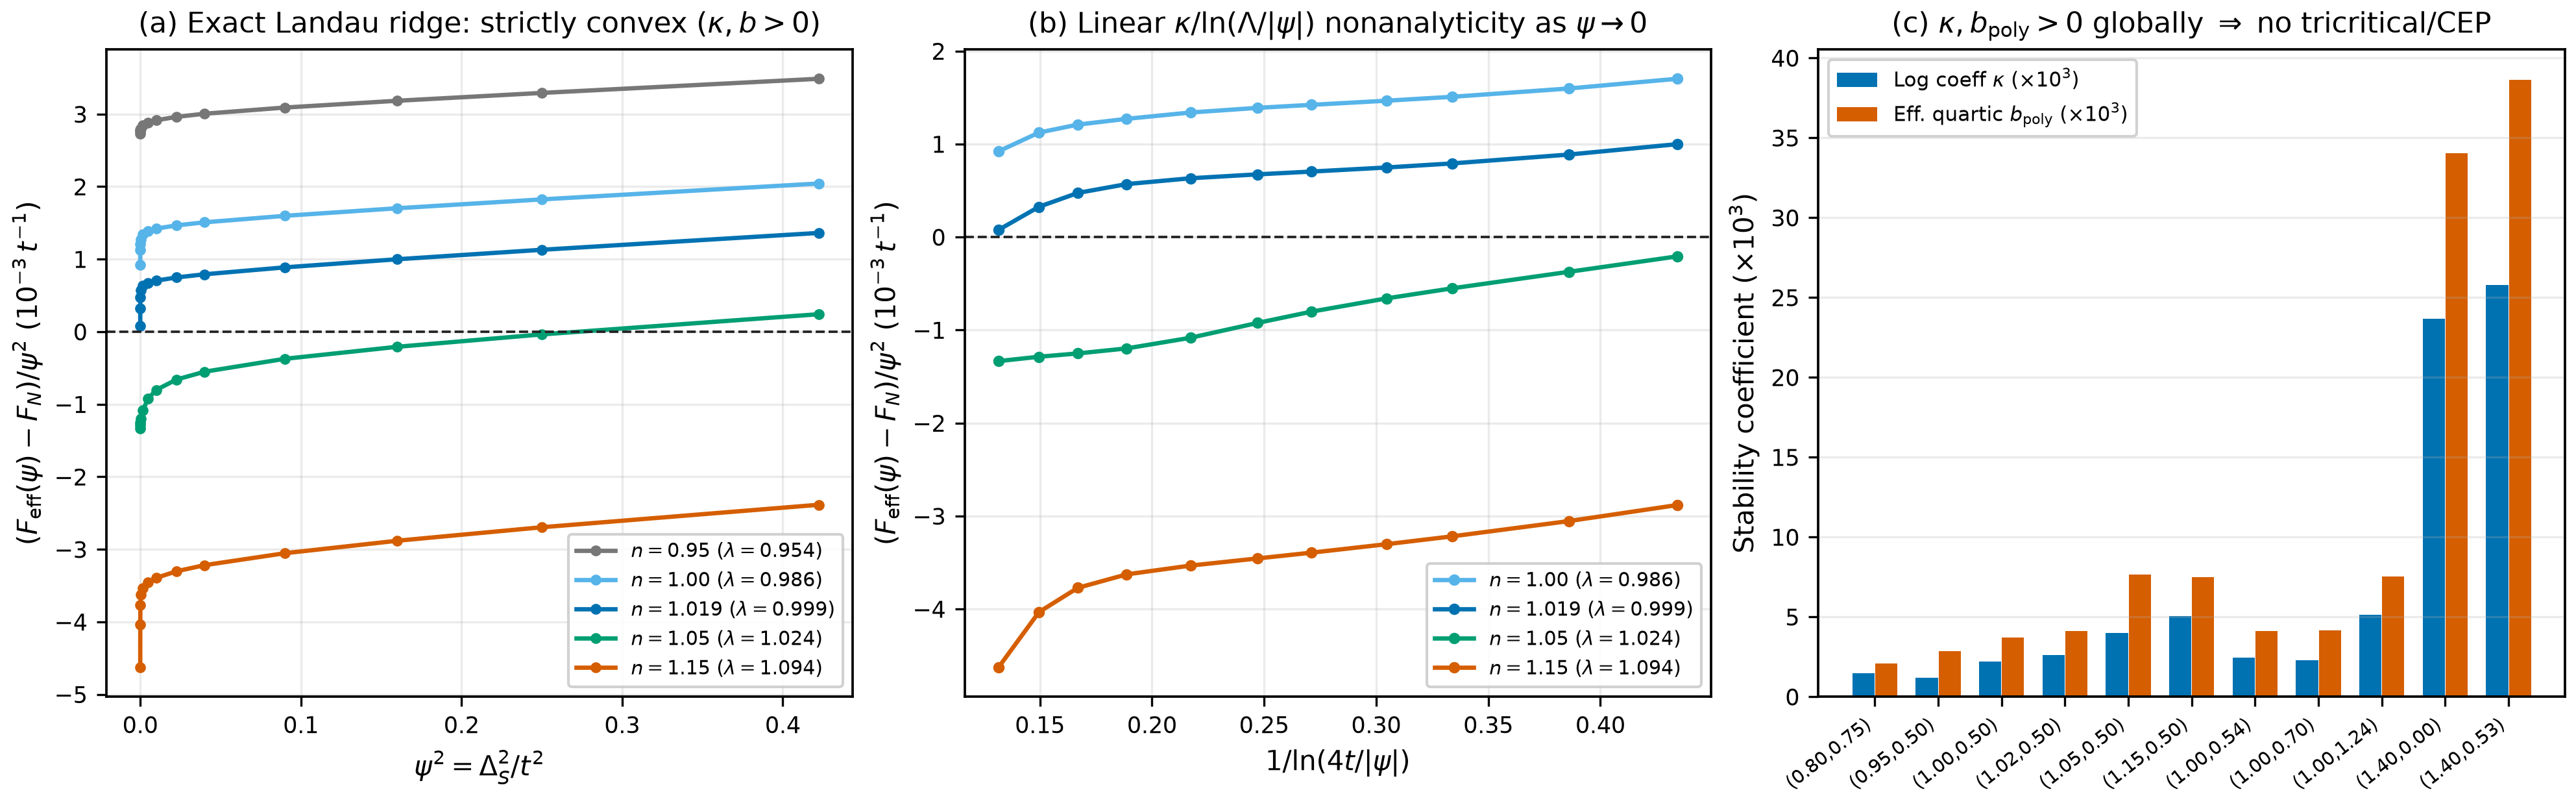
\includegraphics[width=\textwidth]{research/figs/fig07_task4_landau_topology.png}
\caption{Exact constrained Landau potential $F_{\mathrm{eff}}(\psi)-F_N$ along the ridge $r_2=r_3=0$ ($\psi=\Delta_S$): (a)~strict convexity of $(F_{\mathrm{eff}}-F_N)/\psi^2$ across $n_{c,2}=1.0194$ ($U/t=75,\SO/t=0.5$); (b)~linearity against $1/\ln(4t/|\psi|)$ confirming Eq.~\eqref{eq:landau_log}; (c)~global positivity $\kappa, b_{\mathrm{poly}} > 0$ across all tested points, ruling out any tricritical point or first-order coexistence.}
\label{fig:landau_topology}
\end{figure*}

\section{Ground-State Energy Sweeps Against \texorpdfstring{$\SO$}{V\_SO} at \texorpdfstring{$n=1.875$}{n=1.875}}
\label{sec:gse_sweeps}

We next analyze the direct $\SO$-sweep checks executed in \texttt{analysis/\allowbreak ground\_state\_energy\_qpt.py} at the manuscript's high-filling operating point $n=1.875$ across three interaction/correlated-hopping regimes: Case~A ($U/t=75, \Delta_t/t=4.5$, $N_k\in\{201,301,401,601\}$), Case~B1 ($U/t=115, \Delta_t/t=3.5$, $N_k\in\{201,401\}$), and Case~B2 ($U/t=115, \Delta_t/t=4.5$, $N_k\in\{201,401\}$).

\begin{figure*}[t]
\centering
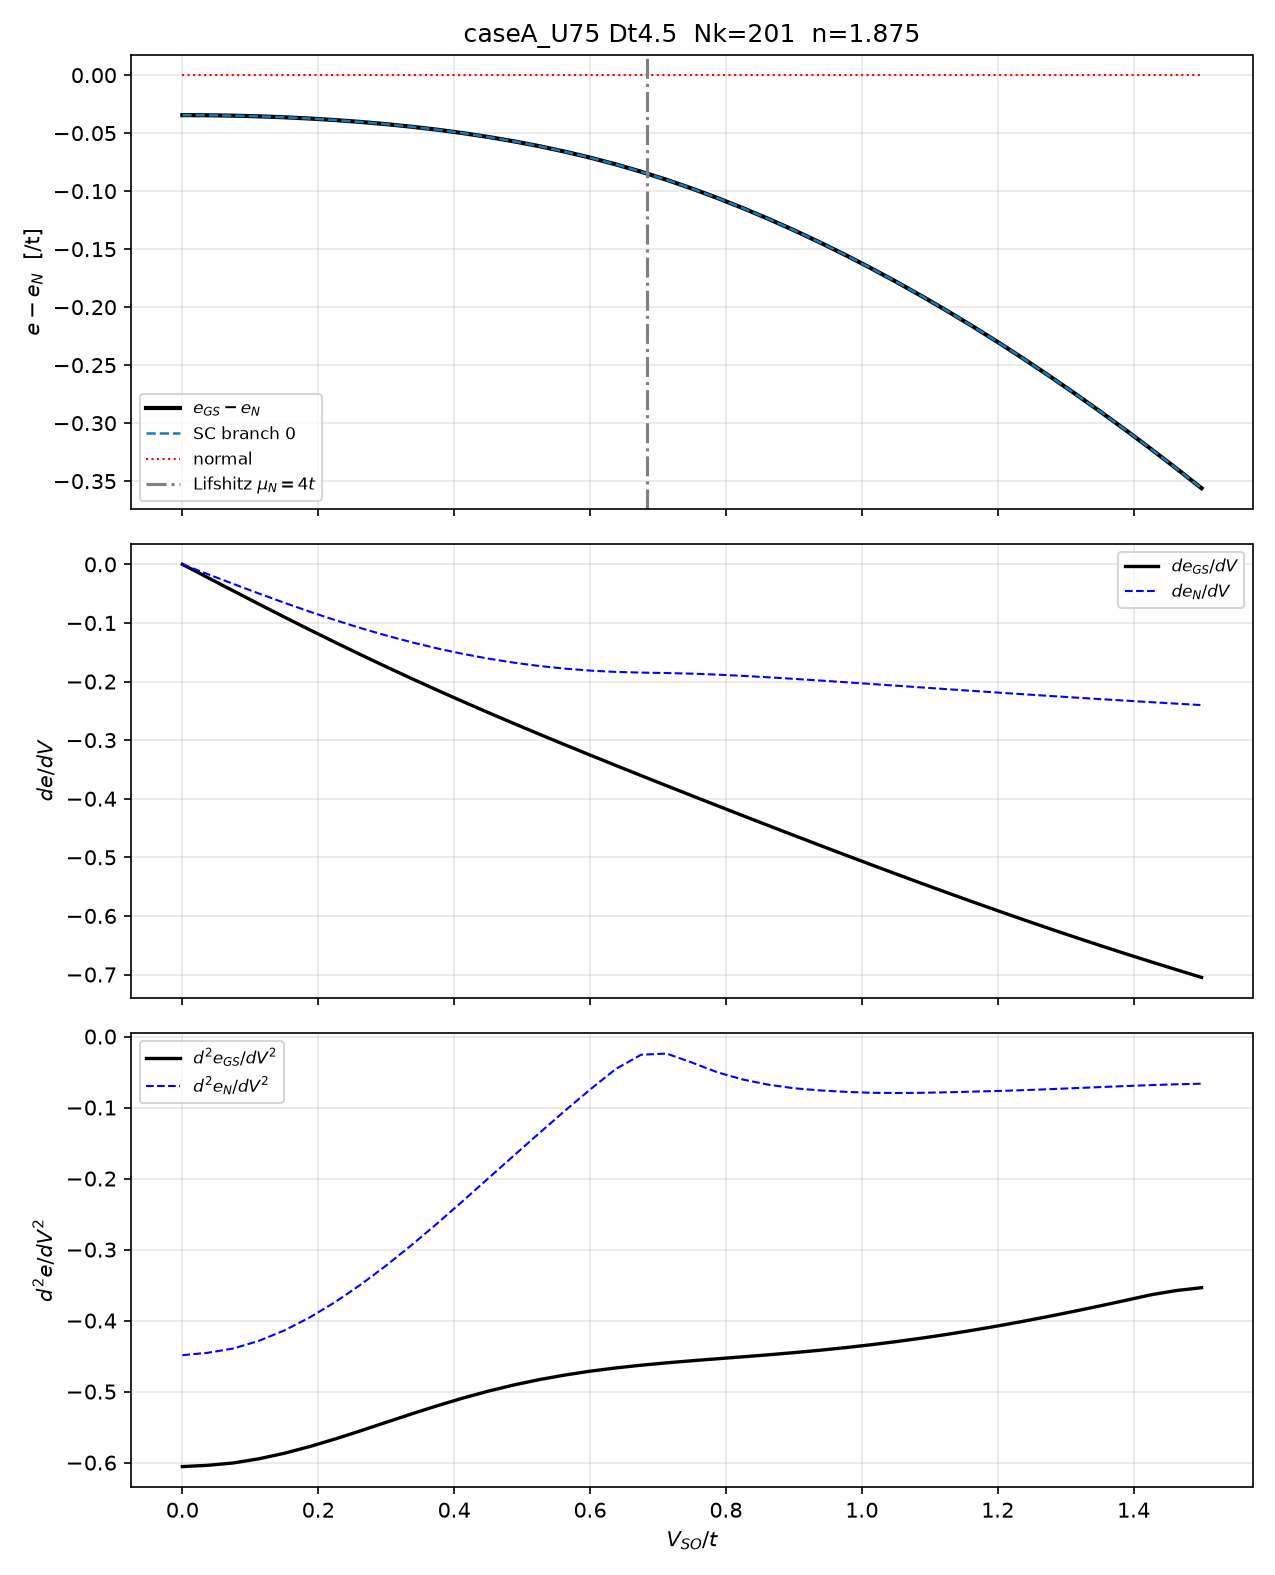
\includegraphics[width=0.326\textwidth]{figs/ground_state_energy_caseA.png}\hfill
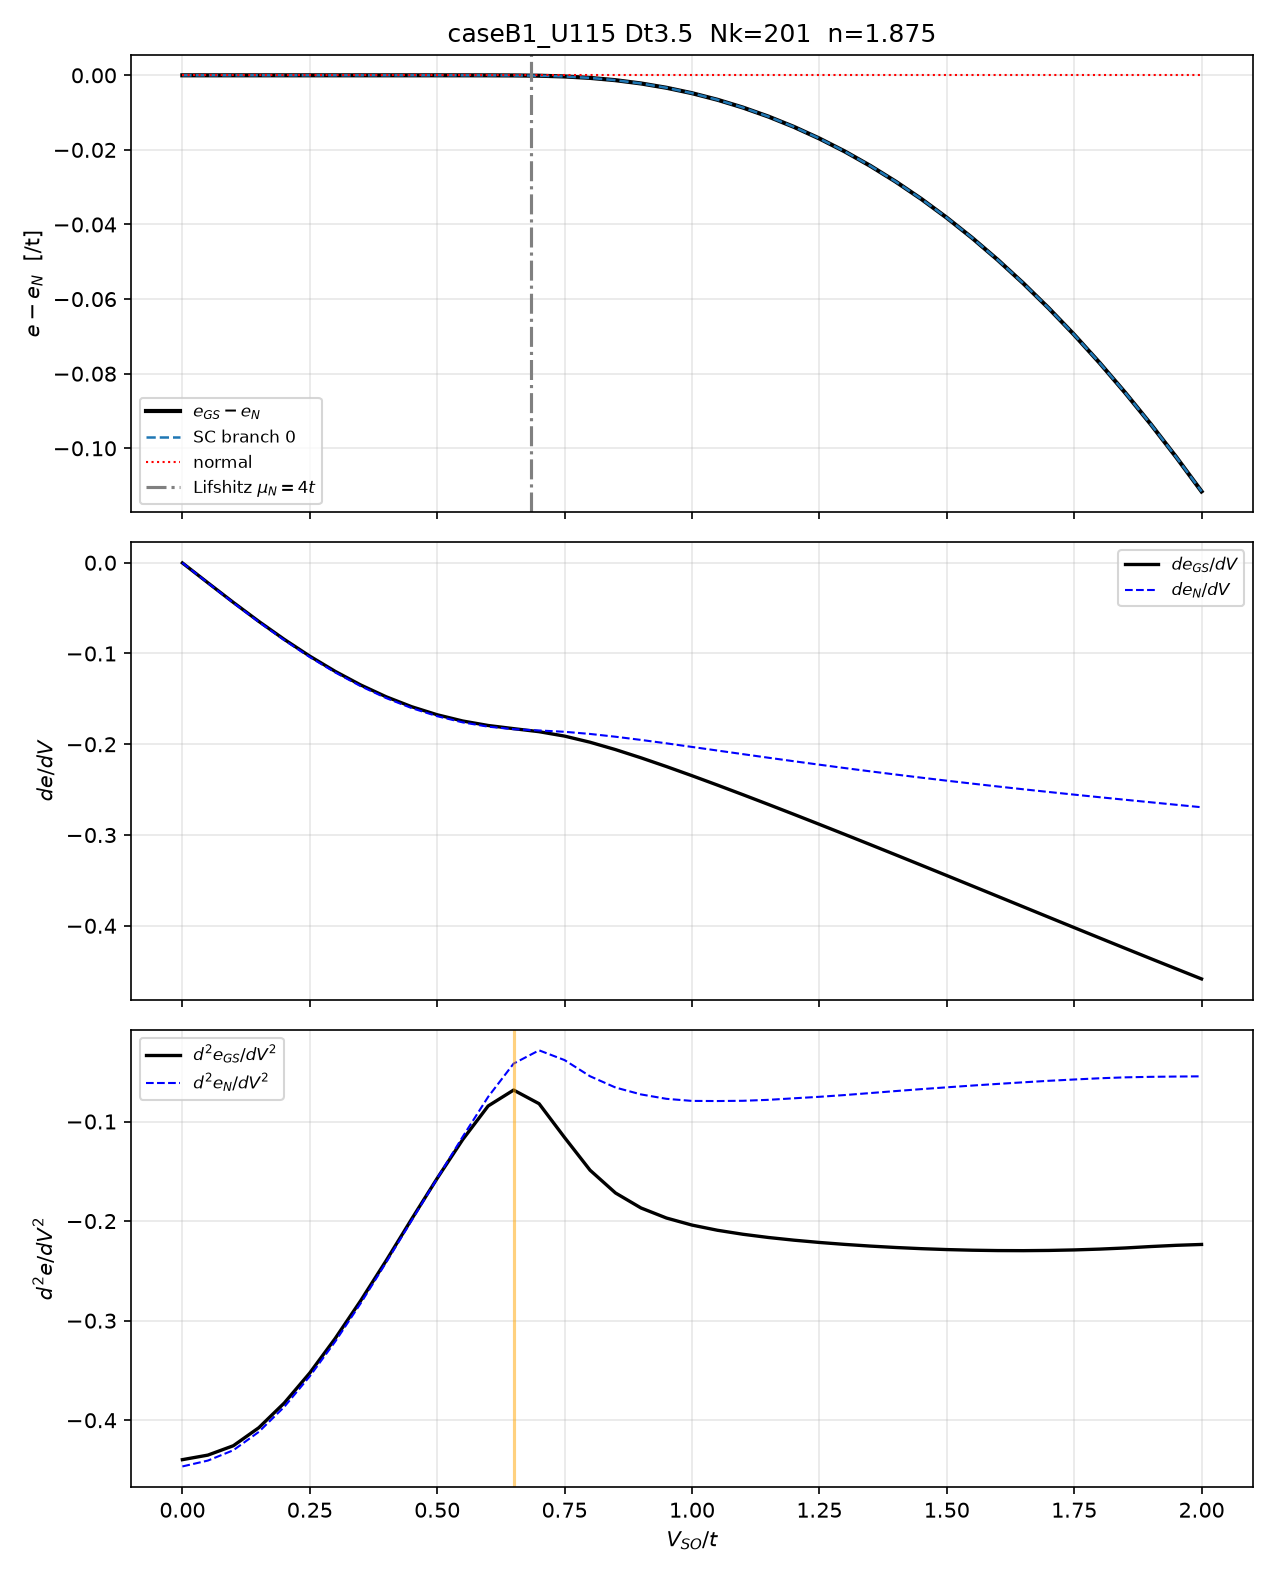
\includegraphics[width=0.326\textwidth]{figs/ground_state_energy_caseB1.png}\hfill
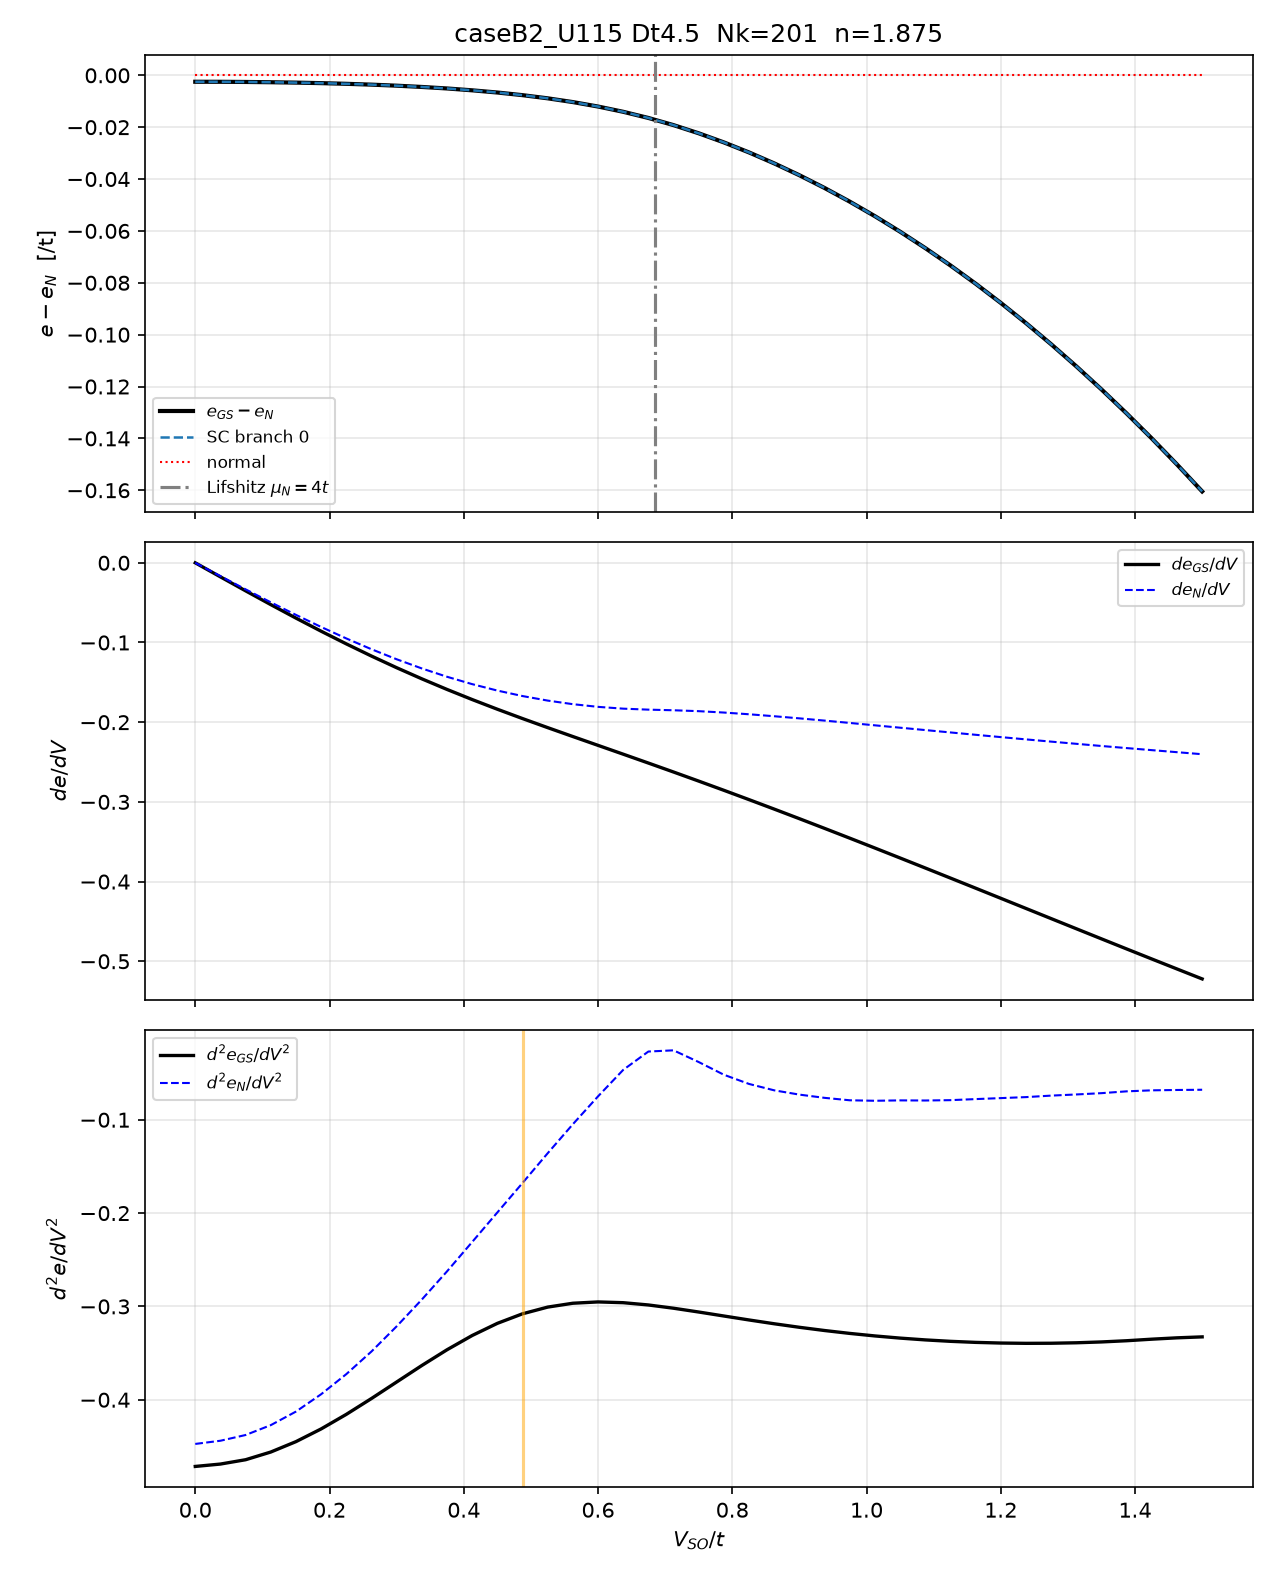
\includegraphics[width=0.326\textwidth]{figs/ground_state_energy_caseB2.png}
\caption{Ground-state energy sweeps from \texttt{analysis/ground\_state\_energy\_qpt.py} ($N_k=201$, $n=1.875$): Case~A ($U/t=75,\Delta_t/t=4.5$, left), Case~B1 ($U/t=115,\Delta_t/t=3.5$, middle), and Case~B2 ($U/t=115,\Delta_t/t=4.5$, right). Top: condensation energy $e_{\mathrm{GS}}-e_N$ showing a single continuous SC branch (vertical dash-dot line marks the normal-state Lifshitz marker $\mu_N=4t$). Middle: first derivative $de/d\SO$ (solid black: SC, dashed blue: normal). Bottom: second derivative $d^2e/d\SO^2$, showing the smooth broad SC inflection versus the sharper normal-state turnover near $\mu_N=4t$ (vertical orange markers in B1/B2 locate numerical smoothed-residual peaks of $d^2e_{\mathrm{GS}}/d\SO^2$, not phase boundaries).}
\label{fig:gse_cases}
\end{figure*}

\begin{table*}[t]
\centering
\caption{Summary of verified ground-state energy sweeps from \texttt{reports/ground\_state\_energy\_qpt.json} ($n=1.875$). $\delta_h/\delta_{2h}$ measures step-doubling stability of numerical derivatives $de_{\mathrm{GS}}/d\SO$ and $d^2e_{\mathrm{GS}}/d\SO^2$.}
\label{tab:gse_verification}
\begin{tabular}{lccccccc}
\toprule
Case & $N_k$ & Branches & $\max|r_{\mathrm{num}}|/N_{\mathrm{tot}}$ & $\frac{d\Omega}{d\mu}$ rel.\ err. & $\SO(\mu_N=4t)/t$ & $\SO(\mu_{\mathrm{SC}}=4t)/t$ & $\delta_h/\delta_{2h}$ ($d_1, d_2$) \\
\midrule
Case A ($U=75,\Delta_t=4.5$)  & 201 & 1 & $2.42\times 10^{-14}$ & $1.11\times 10^{-9}$ & 0.6844 & 0.5485 & ($3.31\times 10^{-4},\; 2.71\times 10^{-3}$) \\
Case A ($U=75,\Delta_t=4.5$)  & 401 & 1 & $5.54\times 10^{-14}$ & ---                  & 0.6901 & 0.5552 & ($3.39\times 10^{-4},\; 2.76\times 10^{-3}$) \\
Case A ($U=75,\Delta_t=4.5$)  & 601 & 1 & $2.79\times 10^{-14}$ & ---                  & 0.6911 & 0.5574 & ($3.41\times 10^{-4},\; 2.78\times 10^{-3}$) \\
Case B1 ($U=115,\Delta_t=3.5$)& 201 & 1 & $3.92\times 10^{-14}$ & $9.89\times 10^{-9}$ & 0.6847 & 0.6880 & ($2.37\times 10^{-3},\; 4.13\times 10^{-2}$) \\
Case B1 ($U=115,\Delta_t=3.5$)& 401 & 1 & $1.81\times 10^{-13}$ & ---                  & 0.6898 & 0.6922 & ($2.40\times 10^{-3},\; 4.45\times 10^{-2}$) \\
Case B2 ($U=115,\Delta_t=4.5$)& 201 & 1 & $3.61\times 10^{-13}$ & $1.74\times 10^{-10}$ & 0.6844 & 0.6958 & ($6.74\times 10^{-4},\; 6.39\times 10^{-3}$) \\
Case B2 ($U=115,\Delta_t=4.5$)& 401 & 1 & $3.45\times 10^{-13}$ & ---                  & 0.6901 & 0.7004 & ($6.91\times 10^{-4},\; 6.61\times 10^{-3}$) \\
\bottomrule
\end{tabular}
\end{table*}

Figure~\ref{fig:gse_cases} and Table~\ref{tab:gse_verification} establish four quantitative facts:
\begin{enumerate}
\item \textbf{Single unique branch:} Across all three parameter sets and up to $N_k=601$, multi-seed continuation recovers $N_b=1$ non-trivial superconducting branch with $e_{\mathrm{GS}} < e_N$ everywhere where pairing is active (the tiny crossings at $V=0.058t, 0.145t$ in $N_k=401$ Case~B1 reflect exponentially suppressed $|\Delta_S|\sim 10^{-4}t$ where $|e_{\mathrm{SC}}-e_N|\lesssim 10^{-10}t$ lies inside floating-point precision).
\item \textbf{Machine-precision thermodynamic consistency:} The number-equation identity~\eqref{eq:dOmega_dmu_total} holds to $\le 3.6\times 10^{-13}$ across every SC point, and independent fixed-$\mu$ solves confirm $d\Omega/d\mu = -N_{\mathrm{tot}}$ to relative error $1.74\times 10^{-10}$--$9.89\times 10^{-9}$.
\item \textbf{Disentangling $\mu_{\mathrm{SC}}=4t$ from $\mu_N=4t$:} In Case~A ($U=75,\Delta_t=4.5$), the superconducting chemical potential crosses $4t$ at $\SO/t = 0.5485$ ($N_k=201$), $0.5552$ ($N_k=401$), and $0.5574$ ($N_k=601$, converging toward $0.5619$ in the continuum), whereas the \emph{normal-state} Fermi-level crossing $\mu_N=4t$ occurs much higher at $\SO/t = 0.6901$ ($N_k=401$, converging to $V_L = 0.6942t$). Figure~\ref{fig:n1875_revalidation} shows that previously reported ``Lifshitz'' coordinates ($0.5487t$, $68.55t$, $118.04t$) were actually $\mu_{\mathrm{SC}}=4t$ crossings on $N_k=201$ meshes; in fixed-$\SO$ $U$-sweeps, $\mu_N$ is completely independent of $U$ ($3.6477t < 4t$ at $\SO=0.5t$; $4.0120t > 4t$ at $\SO=0.7t$), so no normal Lifshitz crossing occurs at all.
\item \textbf{Smooth gapped SC behavior:} Because the Bogoliubov quasiparticle spectrum in Case~A stays strictly gapped ($\min_{\ks}E_{\ks}\ge 0.9374t$ across the entire $\SO\in[0,1.5]t$ sweep, Fig.~\ref{fig:n1875_revalidation}(c)), $e_{\mathrm{GS}}(\SO)$ and its derivatives remain analytic across both $\mu_{\mathrm{SC}}=4t$ and $\mu_N=4t$. By contrast, in Case~B1 ($U=115,\Delta_t=3.5$), the weak pairing tail near $\SO\lesssim 0.65t$ makes $e_{\mathrm{GS}}\approx e_N$, so the SC curve closely follows the sharper normal-state turnover near $\mu_N=4t$.
\end{enumerate}

\begin{figure*}[t]
\centering
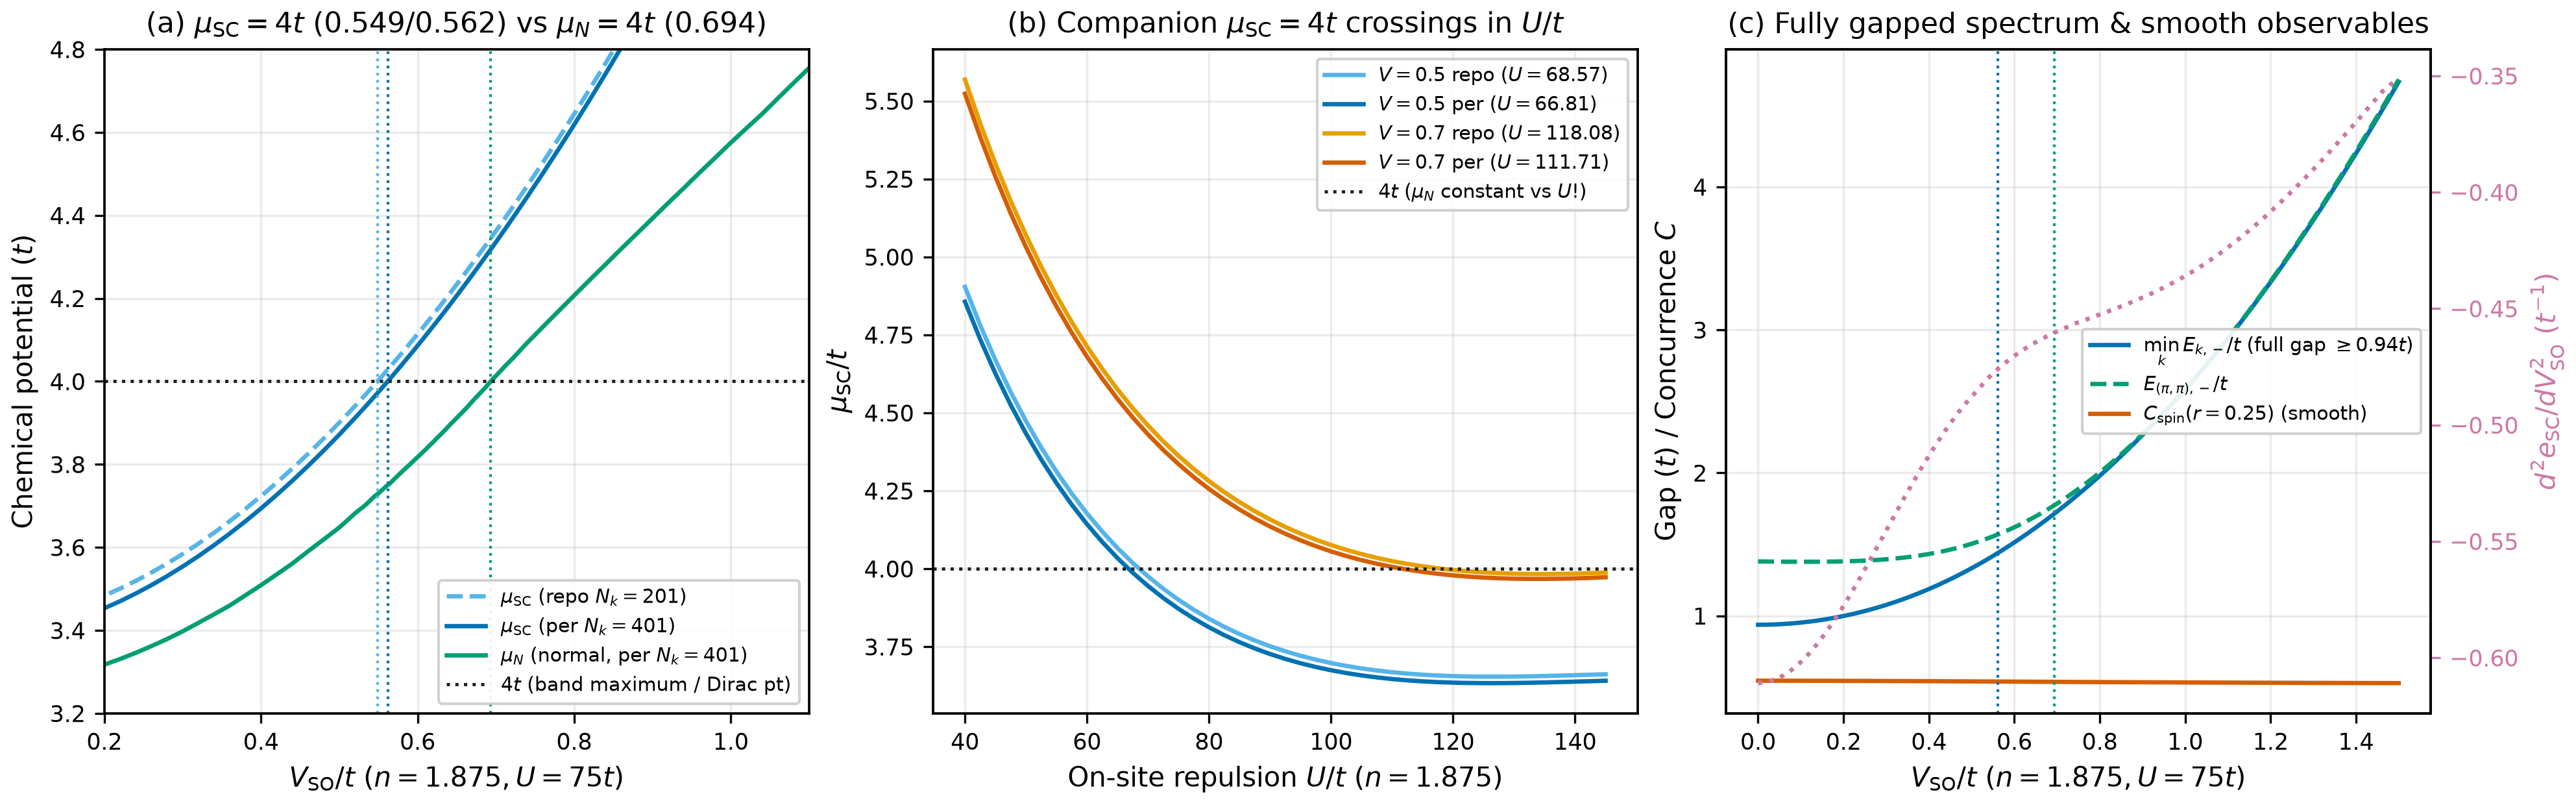
\includegraphics[width=\textwidth]{research/figs/fig10_task6_n1875_revalidation.png}
\caption{Resolution of the $n=1.875$ $\mu=4t$ crossings: (a)~$\mu_{\mathrm{SC}}=4t$ ($0.549t$ on $N_k=201$ repo, $0.562t$ continuum) vs.\ true normal Dirac--Lifshitz $\mu_N=4t$ ($0.694t$); (b)~companion $\mu_{\mathrm{SC}}=4t$ crossings in $U/t$ ($68.57t/66.81t$ at $\SO=0.5t$ and $118.08t/111.71t$ at $\SO=0.7t$), where $\mu_N$ is strictly $U$-independent; (c)~full quasiparticle excitation gap $\min E_{\mathbf{k},-}\ge 0.94t$ guaranteeing analyticity of $d^2e_{\mathrm{SC}}/d\SO^2$ and $C_{\mathrm{spin}}$.}
\label{fig:n1875_revalidation}
\end{figure*}

\section{Analytic Proof of Third-Order Dirac--Lifshitz Scaling at \texorpdfstring{$(\pi,\pi)$}{(pi,pi)}}
\label{sec:dirac_lifshitz}

Why does the normal-state second derivative $d^2e_N/d\SO^2$ in Fig.~\ref{fig:gse_cases} exhibit a smooth V-shaped peak rather than a discontinuous second-order Ehrenfest jump? Expanding Eq.~\eqref{eq:eps_ks} around the Brillouin-zone corner $\mathbf{k} = (\pi - q_x, \pi - q_y)$ yields an isotropic 2D Dirac cone anchored at $E=4t$:
\begin{equation}
\epsilon_{\mp}(\pi - \mathbf{q}) = 4t \mp 2\SO|\mathbf{q}| - t|\mathbf{q}|^2 + \mathcal{O}(q^4).
\label{eq:dirac_cone}
\end{equation}
Because a 2D Dirac cone possesses a linearly vanishing density of states near its apex,
\begin{equation}
N_{\mathrm{cone}}(E) = \int \frac{d^2 q}{(2\pi)^2}\,\delta\!\left(E - 4t \pm 2\SO|\mathbf{q}|\right) = \frac{|E - 4t|}{8\pi \SO^2},
\label{eq:dirac_dos}
\end{equation}
the singular contribution to the $T=0$ grand potential $\delta\Omega_{\mathrm{cone}}(\mu_N) = -\int^{\mu_N} (\mu_N - E)N_{\mathrm{cone}}(E)\,dE$ integrates the linear V-kink twice:
\begin{equation}
\boxed{
\begin{aligned}
\delta\Omega_{\mathrm{cone}}(\mu_N) &\propto \frac{|\mu_N - 4t|^3}{\SO^2} \\
&\quad \times \begin{cases}
-1, & \mu_N < 4t\;\;(\text{inner } \epsilon_- \text{ hole pocket}),\\
+1, & \mu_N > 4t\;\;(\text{inner } \epsilon_+ \text{ electron pocket}).
\end{cases}
\end{aligned}
}
\label{eq:third_order_dirac}
\end{equation}
Unlike a parabolic 2D band edge whose step-function density of states gives $|\mu_N - E_0|^2$ (second-order transition), the $(\pi,\pi)$ Dirac cone gives $|\mu_N - 4t|^3$: a \textbf{third-order} topological Lifshitz transition where $d^2e_N/d\SO^2$ remains continuous with a symmetric cusp while $d^3e_N/d\SO^3$ jumps discontinuously!

\begin{figure*}[t]
\centering
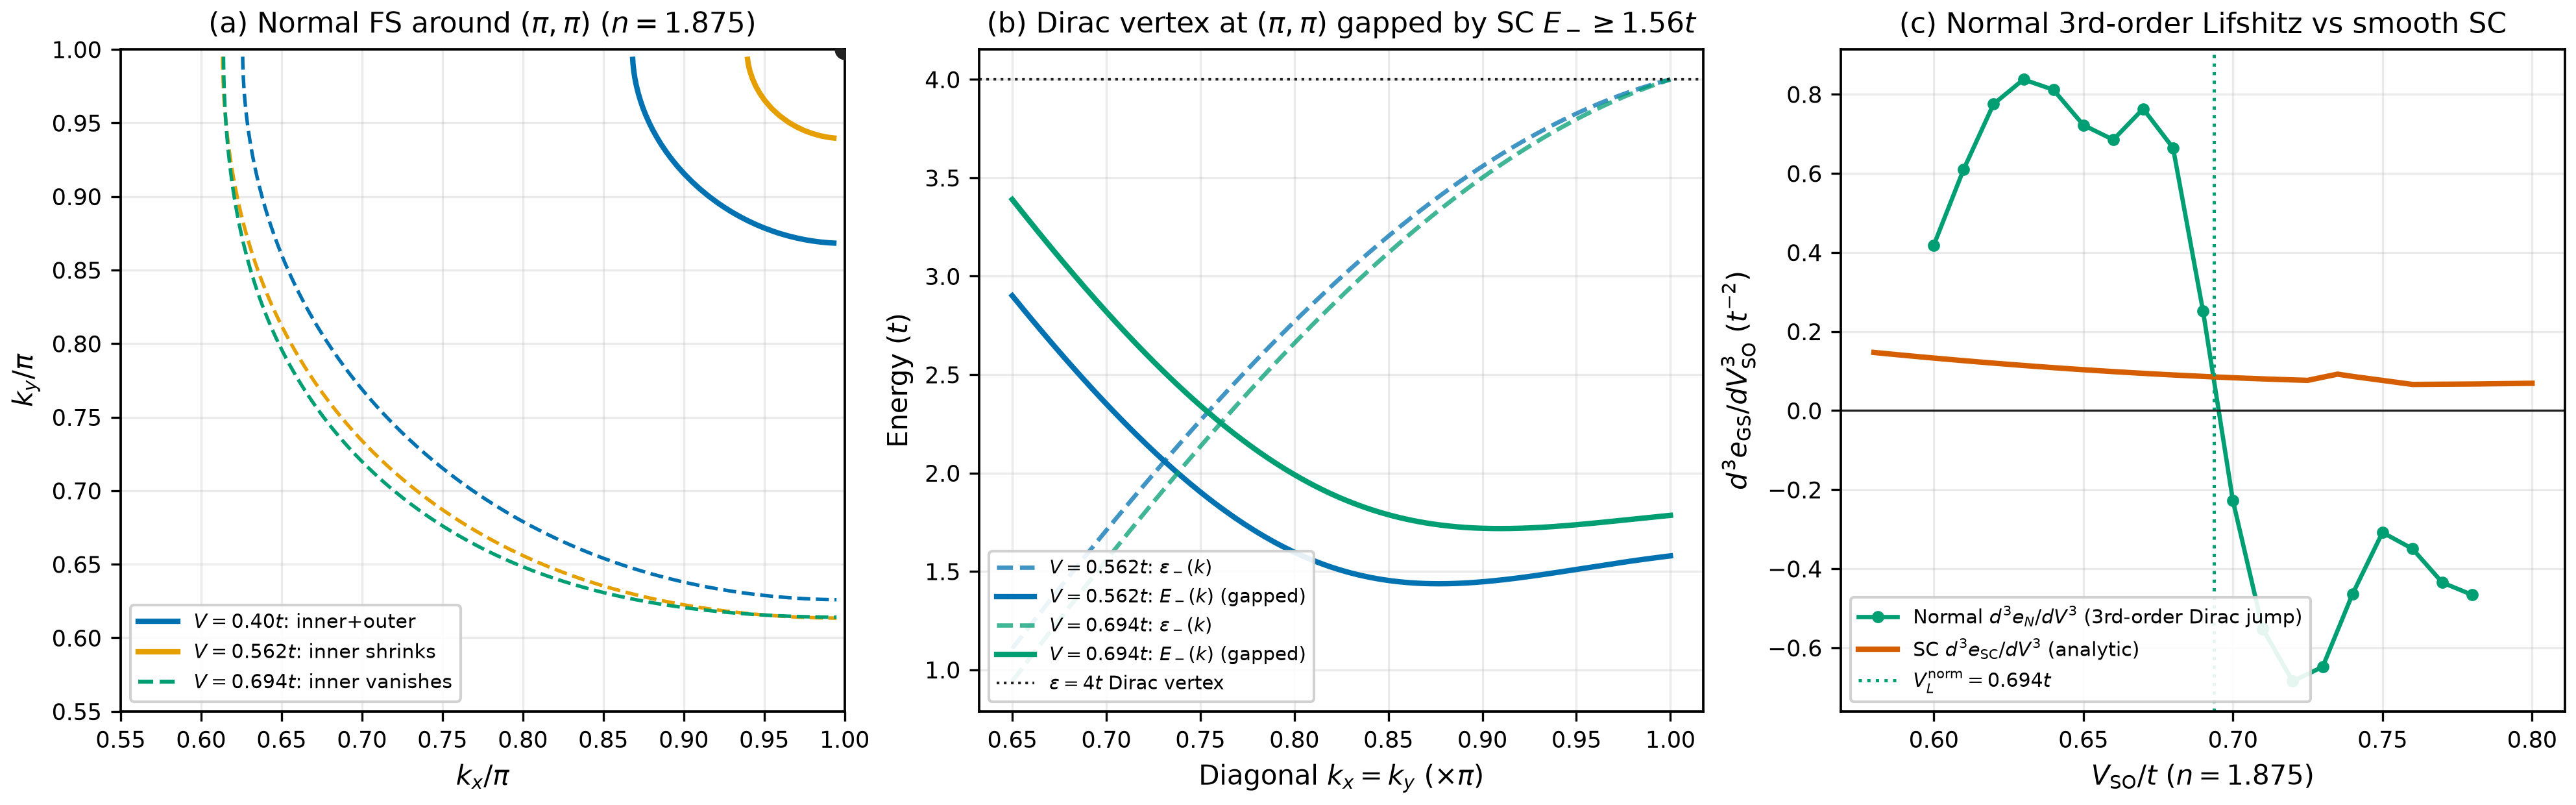
\includegraphics[width=\textwidth]{research/figs/fig11_task6_kspace_topology.png}
\caption{Momentum-space topology and order classification at $n=1.875$: (a)~normal-state Fermi surface near $(\pi,\pi)$ showing the shrinking $\epsilon_-$ hole pocket vanishing at the Dirac apex $V_L = 0.694t$; (b)~diagonal dispersion $\epsilon_-(k_x=k_y)$ reaching $4t$ vs.\ gapped SC quasiparticle dispersion $E_-(k_x=k_y)\ge 1.56t$; (c)~high-precision low-$T$ verification ($N_k=801, T=2\times 10^{-4}t$) showing the discontinuous third-order jump in normal $d^3e_N/d\SO^3$ ($+0.881\to -0.735\,t^{-2}$) contrasted against analytic SC $d^3e_{\mathrm{SC}}/d\SO^3$.}
\label{fig:kspace_topology}
\end{figure*}

Figure~\ref{fig:kspace_topology} verifies Eq.~\eqref{eq:third_order_dirac} directly on $N_k=801$ periodic meshes at $T=2\times 10^{-4}t$: the normal-state $d^2e_N/d\SO^2$ peaks continuously at $-0.00391\,t^{-1}$, while $d^3e_N/d\SO^3$ drops discontinuously from $+0.881\,t^{-2}$ to $-0.735\,t^{-2}$ across $V_L = 0.69426t$. In the superconducting ground state ($U=75t,\Delta_t=4.5t$), pairing opens a large gap $E_-(\pi,\pi)\ge 1.366t$ right at the Dirac apex, leaving $d^3e_{\mathrm{SC}}/d\SO^3$ completely smooth across $V_L$.

\section{Full-Band Density (\texorpdfstring{$n$}{n}) Landscape: Eq.~(28) Energy vs.\ Concurrence}
\label{sec:density_landscape}

Extending the Eq.~(28) energy analysis across the entire electronic filling $n\in(0,2)$ on periodic $N_k=401$ and $N_k=801$ grids clarifies both the global phase structure and the limitations of raw two-qubit concurrence $C(n)$ as a QPT detector (Figs.~\ref{fig:density_landscape} and \ref{fig:density_zooms}, Table~\ref{tab:density_critical}).

\begin{table*}[t]
\centering
\caption{Exact critical pairing densities $n_c$ ($\lambda_+=1$) and normal Fermi-surface topological fillings (van Hove saddles $n_{\mathrm{vH},\pm}$ and $(\pi,\pi)$ Dirac vertex $n_{\mathrm{Dirac},4}$) computed on $N_k=801$ periodic meshes at $\Delta_t/t=4.5$.}
\label{tab:density_critical}
\begin{tabular}{ccccccccc}
\toprule
$\SO/t$ & $U_c(n\to 0^+)/t$ & $n_{\mathrm{sad},-}$ & $n_{\mathrm{vH},-}$ & $n_{\mathrm{Dirac},0}$ & $n_{\mathrm{vH},+}$ & $n_{\mathrm{Dirac},4}$ & $n_c$ ($U=75t$) & $n_c$ ($U=115t$) \\
\midrule
0.0 & 89.999 & 0.00000 & 1.00000 & 1.00000 & 1.00000 & 2.00000 & $\{0.1254,\, 1.1966\}$ & 1.5421 \\
0.4 & 93.531 & 0.00404 & 0.93100 & 1.00000 & 1.06900 & 1.95280 & $\{0.1855,\, 1.0957\}$ & 1.4890 \\
0.5 & 95.459 & 0.00743 & 0.90648 & 1.00000 & 1.09347 & 1.92900 & $\{0.2192,\, 1.0194\}$ & 1.4602 \\
0.7 & 100.422 & 0.01764 & 0.86111 & 1.00000 & 1.13898 & 1.87329 & $\{0.3162,\, 0.8713\}$ & 1.3857 \\
\bottomrule
\end{tabular}
\end{table*}

\begin{figure*}[t]
\centering
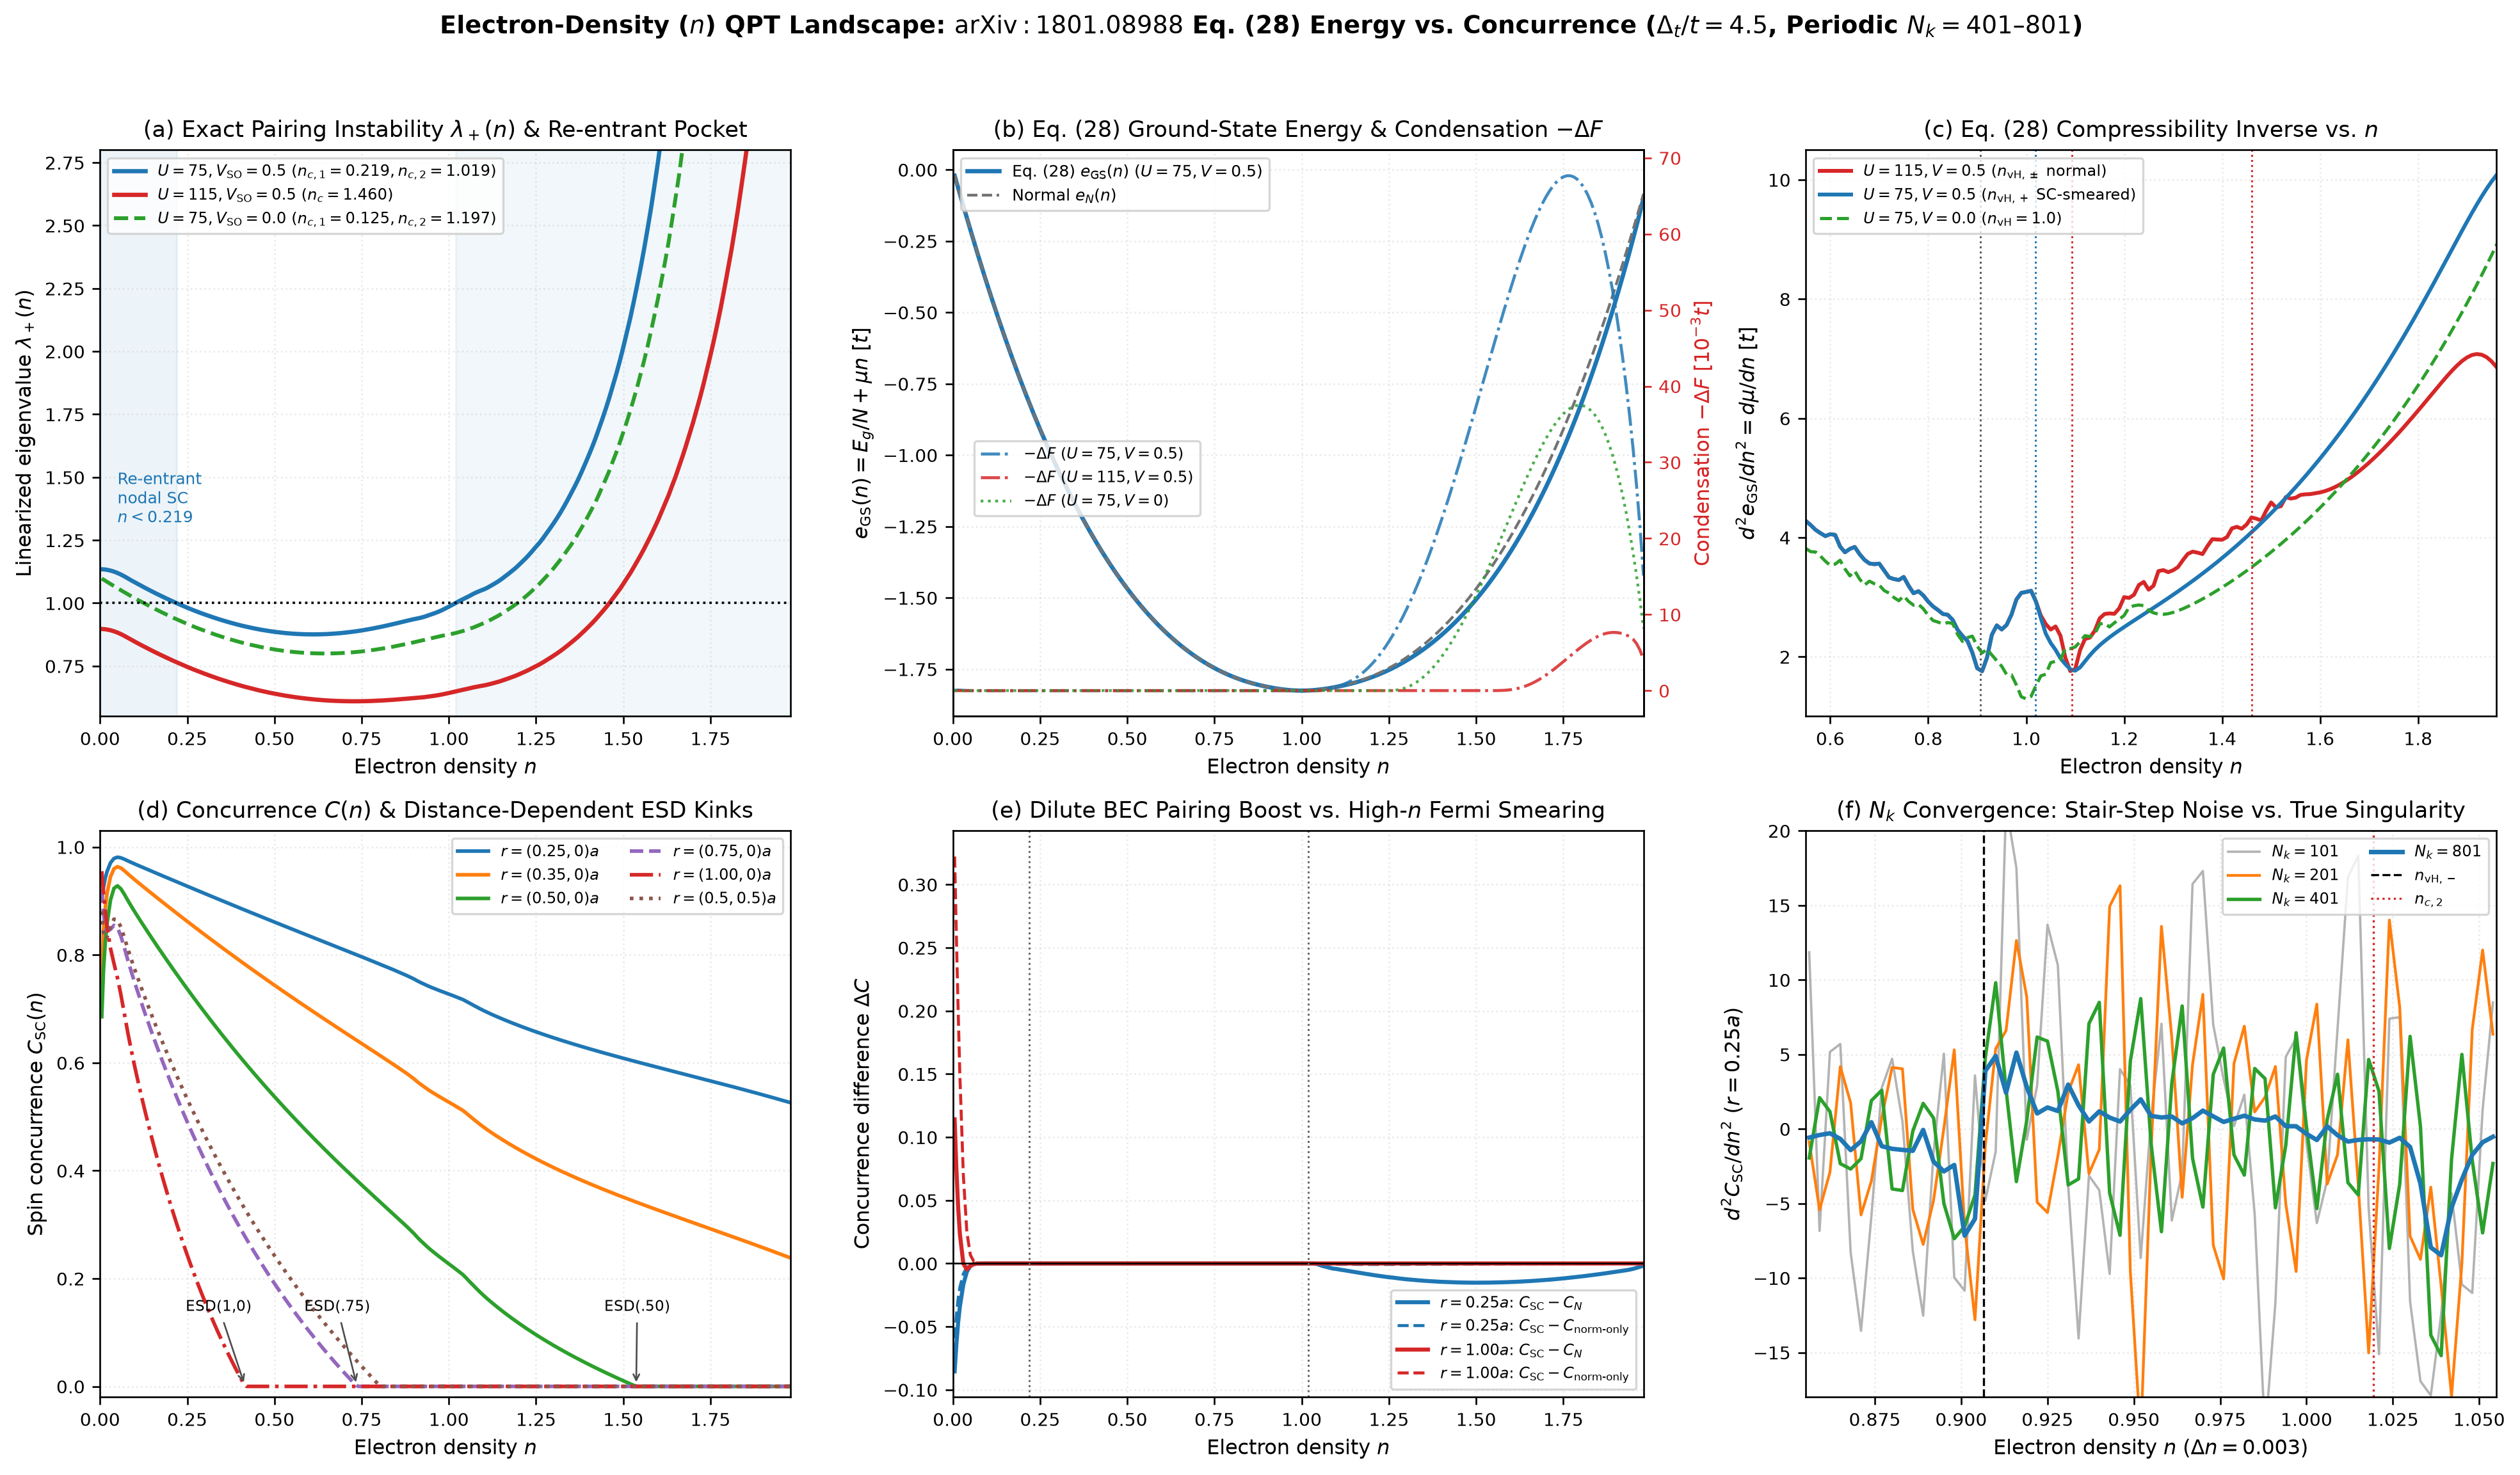
\includegraphics[width=\textwidth]{research/figs/fig13_density_eq28_phase_landscape.png}
\caption{Full-band electron-density QPT landscape ($\Delta_t/t=4.5$, periodic $N_k=401\text{--}801$): (a)~non-monotonic instability eigenvalue $\lambda_+(n)$ revealing both the dilute re-entrant nodal SC pocket ($n<n_{c,1}=0.219$) and the main high-$n$ dome ($n>n_{c,2}=1.019$) at $U/t=75,\SO/t=0.5$; (b)~Eq.~(28) canonical ground-state energy $e_{\mathrm{GS}}(n)=E_g/N+\mu n$ and condensation gain $-\Delta F$; (c)~inverse compressibility $d^2e_{\mathrm{GS}}/dn^2=d\mu/dn$ resolving logarithmic van Hove minima ($n_{\mathrm{vH},\pm}$) in normal regions vs.\ SC smearing; (d)~two-spin concurrence $C_{\mathrm{SC}}(n)$ across separations $r$, dominated by distance-dependent Wootters sudden-death (ESD) kinks; (e)~dilute BEC pairing boost ($r=a$) vs.\ high-density Fermi-smearing suppression; (f)~finite-$N_k$ Fermi-surface stair-step noise in $d^2C_{\mathrm{SC}}/dn^2$.}
\label{fig:density_landscape}
\end{figure*}

\begin{figure*}[t]
\centering
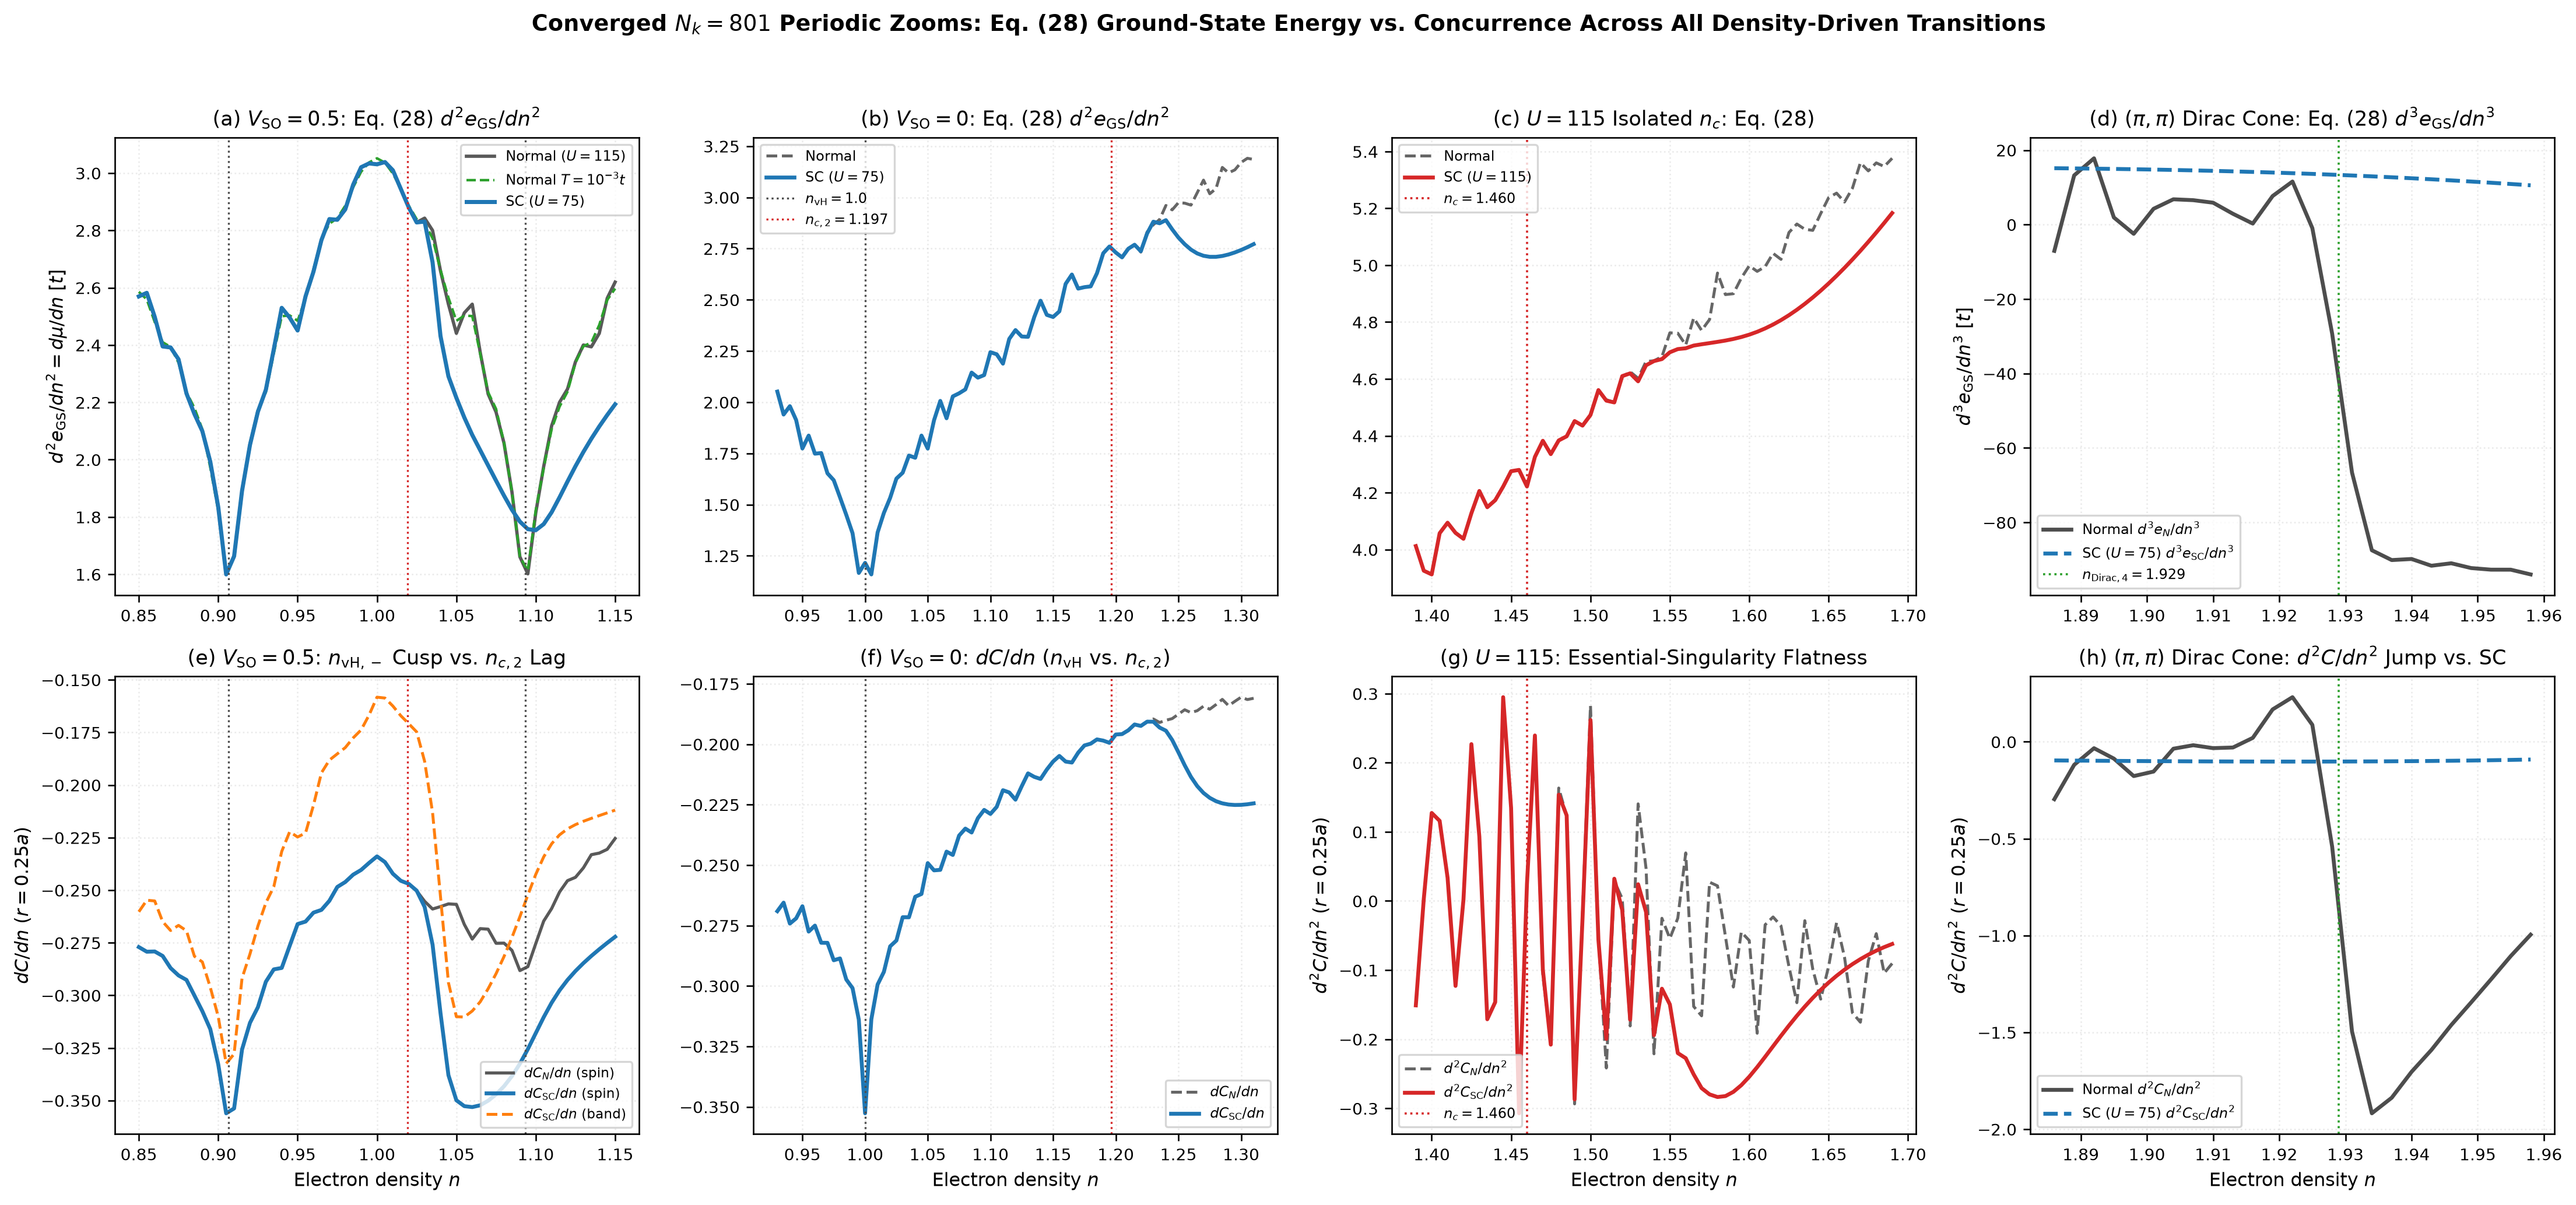
\includegraphics[width=\textwidth]{research/figs/fig14_density_qpt_zooms_eq28_vs_concurrence.png}
\caption{Converged $N_k=801$ zooms comparing Eq.~(28) derivatives (top row) and $r=0.25a$ concurrence derivatives (bottom row) across all density-driven QPT classes: (a,e)~$\SO=0.5t$ normal van Hove saddle ($n_{\mathrm{vH},-}=0.9065$) vs.\ SC-smeared $n_{\mathrm{vH},+}$ and lagged $n_{c,2}$; (b,f)~$\SO=0$ van Hove saddle ($n_{\mathrm{vH}}=1.0$) vs.\ essential-singularity onset ($n_{c,2}=1.197$); (c,g)~$U/t=115$ isolated pairing threshold ($n_c=1.4602$), where both $\Delta F$ and $\Delta C$ remain exponentially flat across $n_c$; (d,h)~$(\pi,\pi)$ Dirac cone ($n_{\mathrm{Dirac},4}=1.9290$), where normal $d^3e_N/dn^3$ ($+11.56\to -91.63\,t$) and $d^2C_N/dn^2$ ($+0.230\to -1.918$) jump together while gapped SC observables remain flat.}
\label{fig:density_zooms}
\end{figure*}

Three structural insights emerge from the density comparison:
\begin{enumerate}
\item \textbf{Dilute re-entrant nodal pocket ($n < n_{c,1}$):} Taking the $n\to 0^+$ limit of Eq.~\eqref{eq:Uc} gives $U_c(0^+) = (2\Delta_t - 4t)\Delta_t|E_{\min}|/t^2 = 95.46t > 75t$ at $\SO=0.5t$. Because $\lambda_+(n)$ is non-monotonic in $n$, the $U=75t$ model supports a dilute nodal ($s_\pm$-like, $\Delta_0\Delta_S < 0$) superconducting pocket below $n_{c,1}=0.2192$ in addition to the main dome above $n_{c,2}=1.0194$, whereas $U=115t > 95.46t$ removes the dilute pocket and leaves a single transition at $n_c=1.4602$.
\item \textbf{Exact detection of van Hove and Dirac QPTs by Eq.~(28):} By Eq.~\eqref{eq:compressibility}, $d^2e_{\mathrm{GS}}/dn^2 = d\mu/dn = 1/g(\mu)$ probes the Fermi-level density of states directly, pinning the logarithmic van Hove cusps ($n_{\mathrm{vH},-}=0.9065$ at $\SO=0.5t$; $n_{\mathrm{vH}}=1.000$ at $\SO=0$) and the third-order $(\pi,\pi)$ Dirac jump ($d^3e_N/dn^3$ stepping from $+11.56t$ to $-91.63t$ at $n_{\mathrm{Dirac},4}=1.9290$, Fig.~\ref{fig:density_zooms}(a--d)). At $n_{c,2}$, however, the BCS essential singularity renders both $\Delta F$ and $\Delta C$ exponentially flat right at $n_c^+$ (e.g., $|\Delta F|<10^{-8}t$ and $|C_{\mathrm{SC}}-C_N|<10^{-5}$ up to $n_c+0.06$ at $U=115t$, Fig.~\ref{fig:density_zooms}(c,g)).
\item \textbf{Limitations of concurrence derivatives:} At $r=0.25a$, over $95\%$ of $C_{\mathrm{SC}}(n)$ originates from normal Fermi-exchange statistics rather than anomalous pairing; moreover, Wootters clipping $C=\max(0,C_{\mathrm{raw}})$ produces artificial sudden-death slope discontinuities at $r$-dependent densities ($n_{\mathrm{ESD}}\in\{0.416,0.737,0.803,1.537\}$ in the spin basis, Fig.~\ref{fig:density_landscape}(d)), and coarse $N_k=101$--$201$ grids generate $\pm 15$--$23$ stair-step noise in $d^2C/dn^2$ [Fig.~\ref{fig:density_landscape}(f)]. Thus Eq.~(28) $e_{\mathrm{GS}}(n)$ provides the unique distance- and basis-independent thermodynamic QPT diagnostic.
\end{enumerate}

\section{Conclusion}
\label{sec:conclusion}

The mathematical framework derived in Eqs.~\eqref{eq:eq28}--\eqref{eq:third_order_dirac} establishes the exact thermodynamic consistency of the ground-state energy checks across the Hubbard--Rashba--correlated-hopping phase diagram. Eliminating the on-shell anomalous counterterm of Eq.~\eqref{eq:eq28} recovers the exact variational functional $F_{\mathrm{eff}}(\Delta_0,\Delta_S,\mu)$ whose Euler--Lagrange equations are the BdG gap equations $(r_1,r_2)=0$ and whose Legendre transform $e_{\mathrm{GS}} = E_g/N + \mu n$ satisfies $d\Omega/d\mu = -N_{\mathrm{tot}}$ and $de_{\mathrm{GS}}/dn = \mu$. Combined with the exact linearized instability threshold $\lambda_+ = 1$, constrained Cooper-logarithmic Landau expansion, and $(\pi,\pi)$ Dirac-cone scaling, these identities prove that the superconducting onset is globally continuous with an essential singularity, rule out candidate first-order transitions and hysteresis artifacts, classify the normal-state $(\pi,\pi)$ Dirac--Lifshitz transition as third order, and confirm that the main $n=1.875$ superconducting protocol regime remains fully gapped and analytic.

\begin{thebibliography}{10}
\bibitem{Hutchinson2018}
J.~Hutchinson, J.~E. Hirsch, and F.~Marsiglio, Phys.\ Rev.\ B \textbf{97}, 184513 (2018).
\bibitem{Sondhi1997}
S.~L. Sondhi, S.~M. Girvin, J.~P. Carini, and D.~Shahar, Rev.\ Mod.\ Phys.\ \textbf{69}, 315 (1997).
\bibitem{Osterloh2002}
A.~Osterloh, L.~Amico, G.~Falci, and R.~Fazio, Nature \textbf{416}, 608 (2002).
\bibitem{Yang2005}
M.-F. Yang, Phys.\ Rev.\ A \textbf{71}, 030302(R) (2005).
\bibitem{Wootters1998}
W.~K. Wootters, Phys.\ Rev.\ Lett.\ \textbf{80}, 2245 (1998).
\bibitem{Oh2004}
S.~Oh and J.~Kim, Phys.\ Rev.\ A \textbf{69}, 054305 (2004).
\bibitem{Oh2005}
S.~Oh and J.~Kim, Phys.\ Rev.\ B \textbf{71}, 144523 (2005).
\bibitem{Yu2009}
T.~Yu and J.~H. Eberly, Science \textbf{323}, 598 (2009).
\end{thebibliography}

\end{document}
